 %%
%% Beginning of file 'sample62.tex'
%%
%% Modified 2018 January
%%
%% This is a sample manuscript marked up using the
%% AASTeX v6.2 LaTeX 2e macros.
%%
%% AASTeX is now based on Alexey Vikhlinin's emulateapj.cls 
%% (Copyright 2000-2015).  See the classfile for details.

%% AASTeX requires revtex4-1.cls (http://publish.aps.org/revtex4/) and
%% other external packages (latexsym, graphicx, amssymb, longtable, and epsf).
%% All of these external packages should already be present in the modern TeX 
%% distributions.  If not they can also be obtained at www.ctan.org.

%% The first piece of markup in an AASTeX v6.x document is the \documentclass
%% command. LaTeX will ignore any data that comes before this command. The 
%% documentclass can take an optional argument to modify the output style.
%% The command below calls the preprint style  which will produce a tightly 
%% typeset, one-column, single-spaced document.  It is the default and thus
%% does not need to be explicitly stated.
%%
%%
%% using aastex version 6.2
\documentclass[]{aastex62}

%% The default is a single spaced, 10 point font, single spaced article.
%% There are 5 other style options available via an optional argument. They
%% can be envoked like this:
%%
%% \documentclass[argument]{aastex62}
%% 
%% where the layout options are:
%%
%%  twocolumn   : two text columns, 10 point font, single spaced article.
%%                This is the most compact and represent the final published
%%                derived PDF copy of the accepted manuscript from the publisher
%%  manuscript  : one text column, 12 point font, double spaced article.
%%  preprint    : one text column, 12 point font, single spaced article.  
%%  preprint2   : two text columns, 12 point font, single spaced article.
%%  modern      : a stylish, single text column, 12 point font, article with
%% 		  wider left and right margins. This uses the Daniel
%% 		  Foreman-Mackey and David Hogg design.
%%  RNAAS       : Preferred style for Research Notes which are by design 
%%                lacking an abstract and brief. DO NOT use \begin{abstract}
%%                and \end{abstract} with this style.
%%
%% Note that you can submit to the AAS Journals in any of these 6 styles.
%%
%% There are other optional arguments one can envoke to allow other stylistic
%% actions. The available options are:
%%
%%  astrosymb    : Loads Astrosymb font and define \astrocommands. 
%%  tighten      : Makes baselineskip slightly smaller, only works with 
%%                 the twocolumn substyle.
%%  times        : uses times font instead of the default
%%  linenumbers  : turn on lineno package.
%%  trackchanges : required to see the revision mark up and print its output
%%  longauthor   : Do not use the more compressed footnote style (default) for 
%%                 the author/collaboration/affiliations. Instead print all
%%                 affiliation information after each name. Creates a much
%%                 long author list but may be desirable for short author papers
%%
%% these can be used in any combination, e.g.
%%
%% \documentclass[twocolumn,linenumbers,trackchanges]{aastex62}
%%
%% AASTeX v6.* now includes \hyperref support. While we have built in specific
%% defaults into the classfile you can manually override them with the
%% \hypersetup command. For example,
%%
%%\hypersetup{linkcolor=red,citecolor=green,filecolor=cyan,urlcolor=magenta}
%%
%% will change the color of the internal links to red, the links to the
%% bibliography to green, the file links to cyan, and the external links to
%% magenta. Additional information on \hyperref options can be found here:
%% https://www.tug.org/applications/hyperref/manual.html#x1-40003
%%
%% If you want to create your own macros, you can do so
%% using \newcommand. Your macros should appear before
%% the \begin{document} command.
%%

\usepackage{graphicx}
\usepackage{float}
\usepackage[caption=false]{subfig}
\usepackage{enumitem}
\usepackage{amsmath}
\listfiles

%\usepackage{natbib}
%\usepackage{pdflscape}

%% AASTeX v6.* now includes \hyperref support. While we have built in specific
%% defaults into the classfile you can manually override them with the
%% \hypersetup command. For example,
%%
%%\hypersetup{linkcolor=red,citecolor=green,filecolor=cyan,urlcolor=magenta}
%%
%% will change the color of the internal links to red, the links to the
%% bibliography to green, the file links to cyan, and the external links to
%% magenta. Additional information on \hyperref options can be found here:
%% https://www.tug.org/applications/hyperref/manual.html#x1-40003

%% If you want to create your own macros, you can do so
%% using \newcommand. Your macros should appear before
%% the \begin{document} command.
%%
\newcommand{\vdag}{(v)^\dagger}
\newcommand\aastex{AAS\TeX}
\newcommand\latex{La\TeX}
\newcommand{\exampleConstant}{0.04}
\newcommand{\degree}{^\circ}
\newcommand{\spitzer}{{\it Spitzer}}
\newcommand{\kepler}{{\it Kepler}}

%% Reintroduced the \received and \accepted commands from AASTeX v5.2
%\received{July 1, 2016}
%\revised{September 27, 2016}
%\accepted{\today}
%% Command to document which AAS Journal the manuscript was submitted to.
%% Adds "Submitted to " the arguement.
%\submitjournal{ApJ}

%% Mark up commands to limit the number of authors on the front page.
%% Note that in AASTeX v6.1 a \collaboration call (see below) counts as
%% an author in this case.
%
%\AuthorCollaborationLimit=3
%
%% Will only show Schwarz, Muench and "the AAS Journals Data Scientist 
%% collaboration" on the front page of this example manuscript.
%%
%% Note that all of the author will be shown in the published article.
%% This feature is meant to be used prior to acceptance to make the
%% front end of a long author article more manageable. Please do not use
%% this functionality for manuscripts with less than 20 authors. Conversely,
%% please do use this when the number of authors exceeds 40.
%%
%% Use \allauthors at the manuscript end to show the full author list.
%% This command should only be used with \AuthorCollaborationLimit is used.

%% The following command can be used to set the latex table counters.  It
%% is needed in this document because it uses a mix of latex tabular and
%% AASTeX deluxetables.  In general it should not be needed.
%\setcounter{table}{1}

%%%%%%%%%%%%%%%%%%%%%%%%%%%%%%%%%%%%%%%%%%%%%%%%%%%%%%%%%%%%%%%%%%%%%%%%%%%%%%%%
%%
%% The following section outlines numerous optional output that
%% can be displayed in the front matter or as running meta-data.
%%
%% If you wish, you may supply running head information, although
%% this information may be modified by the editorial offices.
\shorttitle{NIRCam Lab Stability Studies}
\shortauthors{Schlawin et al.}
%%
%% You can add a light gray and diagonal water-mark to the first page 
%% with this command:
% \watermark{text}
%% where "text", e.g. DRAFT, is the text to appear.  If the text is 
%% long you can control the water-mark size with:
%  \setwatermarkfontsize{dimension}
%% where dimension is any recognized LaTeX dimension, e.g. pt, in, etc.
%%
%%%%%%%%%%%%%%%%%%%%%%%%%%%%%%%%%%%%%%%%%%%%%%%%%%%%%%%%%%%%%%%%%%%%%%%%%%%%%%%%

%% This is the end of the preamble.  Indicate the beginning of the
%% manuscript itself with \begin{document}.

\begin{document}

\title{JWST Noise Floor I: Systematic Error Sources in JWST NIRCam Time Series}

%% LaTeX will automatically break titles if they run longer than
%% one line. However, you may use \\ to force a line break if
%% you desire. In v6.1 you can include a footnote in the title.

%% A significant change from earlier AASTEX versions is in the structure for 
%% calling author and affilations. The change was necessary to implement 
%% autoindexing of affilations which prior was a manual process that could 
%% easily be tedious in large author manuscripts.
%%
%% The \author command is the same as before except it now takes an optional
%% arguement which is the 16 digit ORCID. The syntax is:
%% \author[xxxx-xxxx-xxxx-xxxx]{Author Name}
%%
%% This will hyperlink the author name to the author's ORCID page. Note that
%% during compilation, LaTeX will do some limited checking of the format of
%% the ID to make sure it is valid.
%%
%% Use \affiliation for affiliation information. The old \affil is now aliased
%% to \affiliation. AASTeX v6.1 will automatically index these in the header.
%% When a duplicate is found its index will be the same as its previous entry.
%%
%% Note that \altaffilmark and \altaffiltext have been removed and thus 
%% can not be used to document secondary affiliations. If they are used latex
%% will issue a specific error message and quit. Please use multiple 
%% \affiliation calls for to document more than one affiliation.
%%
%% The new \altaffiliation can be used to indicate some secondary information
%% such as fellowships. This command produces a non-numeric footnote that is
%% set away from the numeric \affiliation footnotes.  NOTE that if an
%% \altaffiliation command is used it must come BEFORE the \affiliation call,
%% right after the \author command, in order to place the footnotes in
%% the proper location.
%%
%% Use \email to set provide email addresses. Each \email will appear on its
%% own line so you can put multiple email address in one \email call. A new
%% \correspondingauthor command is available in V6.1 to identify the
%% corresponding author of the manuscript. It is the author's responsibility
%% to make sure this name is also in the author list.
%%
%% While authors can be grouped inside the same \author and \affiliation
%% commands it is better to have a single author for each. This allows for
%% one to exploit all the new benefits and should make book-keeping easier.
%%
%% If done correctly the peer review system will be able to
%% automatically put the author and affiliation information from the manuscript
%% and save the corresponding author the trouble of entering it by hand.

\correspondingauthor{Everett Schlawin}
\email{eas342 AT EMAIL Dot Arizona .edu}

\author[0000-0001-8291-6490]{Everett Schlawin}
\affiliation{Steward Observatory \\
933 North Cherry Avenue \\
Tucson, AZ 85721, USA}

\author{Jarron Leisenring?}
\affiliation{Steward Observatory \\
933 North Cherry Avenue \\
Tucson, AZ 85721, USA}

\author{Karl Misselt?}
\affiliation{Steward Observatory \\
933 North Cherry Avenue \\
Tucson, AZ 85721, USA}

\author{Thomas Beatty?}
\affiliation{Steward Observatory \\
933 North Cherry Avenue \\
Tucson, AZ 85721, USA}

\author{Thomas P Greene?}
\affiliation{NASA Ames Research Center \\
Space Science and Astrobiology Division \\
Moffett Field, CA 94035, USA}

\author{Michael McElwain}
\affiliation{NASA Goddard Space Flight Center \\
Exoplanets and Stellar Astrophysics Laboratory \\
Greenbelt, MD 20771, USA}

\author{Marcia Rieke}
\affiliation{Steward Observatory \\
933 North Cherry Avenue \\
Tucson, AZ 85721, USA}


%% Note that the \and command from previous versions of AASTeX is now
%% depreciated in this version as it is no longer necessary. AASTeX 
%% automatically takes care of all commas and "and"s between authors names.

%% AASTeX 6.1 has the new \collaboration and \nocollaboration commands to
%% provide the collaboration status of a group of authors. These commands 
%% can be used either before or after the list of corresponding authors. The
%% argument for \collaboration is the collaboration identifier. Authors are
%% encouraged to surround collaboration identifiers with ()s. The 
%% \nocollaboration command takes no argument and exists to indicate that
%% the nearby authors are not part of surrounding collaborations.

%% Mark off the abstract in the ``abstract'' environment. 
\begin{abstract}

JWST transmission and emission spectra of transiting exoplanets will provide invaluable glimpses of exoplanet atmospheres.
These spectra will reveal the composition and temperature structure at a level never achieved before.
This promising science from JWST, however, will require exquisite precision and understanding of systematic errors that can impact the time series of planets crossing in front of and behind their host stars.
This is especially true if JWST is used to search for biosignatures in temperate atmospheres and other weak signatures.
Here, we provide estimates of the noise sources affecting JWST NIRCam time-series data.
Correlated electronic noise (1/f noise) in the detectors can limit the precision of grism time series for a given frame (230 ppm to 1000 ppm depending on the extraction method), but will average down like $\sqrt{N}$ for $N$ frames/reads.
Care should be taken to include as many frames as possible per visit to reduce this 1/f noise source: thus, we recommend the smallest detector subarray sizes one can tolerate, 4 output channels and readout modes that minimize skipped frames (RAPID or BRIGHT2).
We also describe a covariance weighting scheme that can significantly lower the contributions from 1/f noise as compared to sum extraction.
Pointing jitter and high gain antenna moves on top of the detectors' subpixel crosshatch patterns will produce relatively small variations $\lesssim 10$ ppm, before they are corrected.
In contrast to the HST WFC3 detectors, persistence due to charge trapping will have a negligible effect on time series.
\end{abstract}

%% Keywords should appear after the \end{abstract} command. 
%% See the online documentation for the full list of available subject
%% keywords and the rules for their use.
\keywords{Concept: Astronomical detectors --- Concept: Exoplanet atmospheres --- Concept: Near infrared astronomy}

%% From the front matter, we move on to the body of the paper.
%% Sections are demarcated by \section and \subsection, respectively.
%% Observe the use of the LaTeX \label
%% command after the \subsection to give a symbolic KEY to the
%% subsection for cross-referencing in a \ref command.
%% You can use LaTeX's \ref and \label commands to keep track of
%% cross-references to sections, equations, tables, and figures.
%% That way, if you change the order of any elements, LaTeX will
%% automatically renumber them.

%% We recommend that authors also use the natbib \citep
%% and \citet commands to identify citations.  The citations are
%% tied to the reference list via symbolic KEYs. The KEY corresponds
%% to the KEY in the \bibitem in the reference list below. 

\section{Introduction} \label{sec:intro}

JWST will provide powerful new measurements of exoplanet atmospheres with spectroscopy from 0.6 to 28 $\mu$m
\citep{beichman2014pasp,greene2016jwst_trans,howe2017informationJWST,barstow2015jwstSystematics,schlawin2018JWSTforecasts}.
The sensitivity of JWST combined with its unprecedented wavelength coverage on exoplanets will enable it to measure the abundance of carbon-bearing molecules (CO, CO$2$ and CH$_4$) as well as study cooler, smaller planets than previously characterized.

JWST has also been considered for observations of potentially habitable Earth-like planets that orbit their stars at a distance where water could be in liquid form on their surface.
The TRAPPIST-1 system \citep{gillon2016trappist1Discovery,gillon2017trappist-1sevenp} presents an exciting opportunity to study Earth-sized stars orbiting a 0.1~R$_\odot$ M-type star.
By putting together 10 to 30 transits, it will be possible to collect enough photons to detect CO$_2$ \citep{barstow2016trappist1habitable,krissansen-totton2018trappist1eJWST,lustig-yaeger2019detectabilityTRAPPIST-1}.
Optimistically, 30 transits may contain enough photons to detect O$_3$ in the atmosphere of TRAPPIST-1 d with JWST if clouds have a minimal impact on its atmosphere \citep{barstow2016trappist1habitable}.
More detailed modeling of atmospheric evolution indicates that biogenic oxygen may be too difficult to detect with any JWST instrument but desiccated oceans may produce detectable abiogenic oxygen \citep{lustig-yaeger2019detectabilityTRAPPIST-1}.
Alternatively, 10 transits of TRAPPIST-1e could be sufficient if the planet's atmosphere has CO$_2$ and CH$_4$ biosignatures similar to early-Earth \citep{krissansen-totton2018trappist1eJWST}.
A critical question in studying planets like TRAPPIST-1 d/e, however, is whether photon-limited performance is possible with JWST observations.
For difficult biosignatures, noise levels less than 10 ppm (parts per million) are required and this value shrinks in the presence of clouds.

Experience with the \textit{Hubble Space Telescope} (HST), \spitzer, and \kepler\ shows that many systematics can affect high precision time series and prevent photon-limited performance unless corrected \citep[e.g.][]{beichman2014pasp}.
Many of these effects are detector-related including charge trapping on HST's detector \citep{berta2012flat_gj1214,zhou2017chargeTrap}, intra-pixel sensitivity on the short wavelength bands of \spitzer\ IRAC \citep{moralesCalderon2006LdwarfsWeatherIPC} and sensitivity to pointing jitter with \kepler\footnote{https://keplerscience.arc.nasa.gov/K2/Performance.shtml} \citep[e.g.][]{vanderburg2014twoWheeledKeplerPhot,beichman2014pasp}.

The NIRCam instrument \citep{rieke2005nircamSPIE} contains a slitless grism mode with its long wavelength (LW) channel \citep{greene2017jatisNIRCam}.
This slitless grism mode is analogous to the WFC3 grism on HST that has been successfully employed on many transiting planets \citep[e.g.][]{deming13,kreidberg2014wasp43,sing2016continuum,wakeford2017hatp26}.
The NIRCam grism mode will collect moderate resolution R$\sim$1100-1700 spectra over the wavelength range from 2.4 to 5.0~$\mu$m.
This grism mode can be used simultaneously with short wavelength weak lens imaging or (in future cycles) the Dispersed Hartmann Sensor mode \citep{schlawin2017dhs}. If it becomes an approved and implemented mode, the DHS will permit spectroscopy simultaneous from 1.0 to 2.0~$\mu$m because of a dichroic beamsplitter that divides the light from NIRCam into two different channels.
The DHS mode will permit time series spectroscopy on very bright targets ($K_S \sim 1$) inaccessible by other modes.

Given the finite lifetime of the JWST mission set by onboard fuel, it is important to understand the systematic errors before launch to maximize the science return of the observatory.
We discuss the major sources of systematic errors that can affect the NIRCam instrument.
Parallel efforts to characterize other instrument's noise sources are being carried out, such as with MIRI's detectors \citep{matuso2019siAsDetectorStability}.

Section \ref{sec:knownEffects} lists the known systematic effects that can impede high precision time series and increase the noise above the photon noise.
Sections \ref{sec:preAmp} through \ref{sec:persistence} detail these noise contributions.
We conclude in Section \ref{sec:Conclusion} that 1/f noise is the largest systematic error followed by subpixel sensitivity, while the dominant HST-related systematic should have a relatively minor impact for JWST.

\section{List of Known Detector Effects}\label{sec:knownEffects}
An ideal HgCdTe detector simply counts the photons incident on its surface (as described in section \ref{sec:detectorPrimer}).
However, there are many non-ideal effects that can affect the stability of a light curve of a transiting exoplanet.
Here, we review many of the known noise sources that could impact the stability of a time series beyond photon counting statistics. The known detector effects that can impact stability are listed briefly and then discussed in more detail as related to the JWST NIRCam detectors.

\begin{itemize}[noitemsep]
	\item \textbf{Pre-amplifier reset offsets:} (an ASIC-related effect) 
The resets cause discontinuities in the pedestal level of all pixels between frames.
Pre-amp resets can also appear in slope images (DN/second) because NIRCam's amplifiers are reset once per frame (not once per integration).
This is an effect where averaging over more pixels does not decrease the noise, but reference pixel or background subtraction can efficiently remove the pre-amp offsets.
These are discussed further in Section \ref{sec:preAmp}.
	\item \textbf{Amplifier Boundary Discontinuities} The NIRCam detectors can be read out in full frame, stripe and window modes. The full frame and stripe modes make use of 4 amplifiers that can record or reset the accumulated electrons using 4 pixels simultaneously in parallel. The parallel operation of the amplifiers reduces the frame time and reset time by a factor of 4 but can introduce subtle voltage biases between regions of the detector. If these voltage biases are not corrected, they can potentially introduce discontinuities in a spectrum, which crosses amplifier boundaries.
	The amplifier boundary discontinuities are a consequence of the pre-amplifier reset offsets described above.
	\item \textbf{1/f noise:} The JWST HgCdTe readout electronics have a p-type metal-oxide semiconductor field-effect transistor (PFET) source follower that introduces noise to the images as well as DC biases in the ASIC electronics \citep{rauscher2011irsSquared}.
	This is a noise source where most of the noise power is concentrated at low frequencies.
	1/f noise causes spatial correlations primarily in the fast-read direction (along detector rows). It is highly correlated between amplifiers, suggesting that it is caused by a common reference voltage. 1/f noise can be reduced by subtracting the values from background pixels or reference pixels.
	\item \textbf{Intrapixel sensitivity:} Telescope pointing drifts and jitter can impact the amount of flux measured if the response within a pixel is not perfectly uniform.
	This has a particularly strong impact on the time series from the Spitzer IRAC instrument \citep{ingalls2016spitzerRepeatability}.
	It can also appear on JWST detectors because the sub-pixel flat field is not uniform.
	Crosshatching patterns on HgCdTe detectors, which all JWST near-infrared instruments use, exist at the sub-pixel level  \citep{shapiro2018crosshatch,ninan2019crosshatchHPF}
	\item \textbf{Even/odd offsets:} Alternating columns have different bias levels. Additionally, there are offsets between columns that can change from frame to frame, especially on NIRCam's LW detector.
	These can be reduced with reference pixels or background subtraction.
	\item \textbf{kTC noise:} Each reset at the beginning of an integration introduces thermal noise associated with the unknown amount of charge stored in a pixel at the reset voltage level.
	Fortunately, the bias offset produced by kTC noise will easily subtract out when fitting a slope image from multiple samples up the ramp.
	This noise would only become relevant when attempting to make use of the first group of a ramp, such as when only 1 group is commanded.
	\item \textbf{Detector Temperature Fluctuations:} The JWST detectors are sensitive to temperature changes on the focal plane arrays. For example, laboratory tests show that 100 mK temperature fluctuations can result in $\sim$80 ADU changes on the detector that are not corrected by reference pixels \citep{hall2005jwstArrays}. Fortunately, the detectors are actively thermally controlled to keep the temperature fluctuations to mostly $\lesssim$ 1 mK.
The one exception is that the NIRCam LW A-side detector (A5) exhibited $\sim$ 20 min oscillations with an amplitude of 15-20 mK when using the Temperature Monitor Control (TMC) 1 active thermal control.
Fortunately, the TMC 2 control does not undergo these oscillations and will be employed in orbit.
If necessary, the effect of temperature fluctuations can be calibrated to $\pm 1 e^-$ for excursions less than $\pm$ 50 mK \citep{hall2005jwstArrays}.
	\item \textbf{ASIC Temperature Fluctuations:} The ASIC temperature will change depending on the operating mode. For example, in the CV3 stability test, the temperature of the A ASIC changed by $\sim$80 mK when the readout mode was switched from full frame to subarray.
	This temperature change is expected to be smaller in flight due to adjustments in the operations to run all four amplifiers regardless of how many are used to collect science data.
	\item \textbf{Elevated Columns} There is correlated noise along a column in many frames. These elevated columns can move with time.
	\item \textbf{Random Telegraph Noise (RTN)} Some of the pixels will exhibit spontaneous changes jumps in signal even with no illumination. Fortunately, RTN appears in only $\sim$1000 pixels out of 4$\times 10^6$ on the array.
	\item \textbf{Detector Fringing} \textbf{\textcolor{red}{Is there a good citation?}} The thin $\sim 5\mu$m layers of the H2RG detectors will cause interference patterns on the array due to constructive and destructive interference of light at wavelengths similar to the thickness of the layers. If the detector fringe pattern changes with time, it will change the throughput of a grism image.
	\item \textbf{Charge Trapping} A major correlated error source on HST WFC3 is the ``hook effect'' \citep{berta2012flat_gj1214}.
	The hook effects is due to charge can be trapped within the detector's depletion region, initially lowering the flux, and then released at later times thereby increasing the flux \citep{zhou2017chargeTrap}.
	JWST's NIRCam instrument has very lower rates of persistence ($<$1 DN/sec) at 100 seconds after saturation \citep{leisenring2016persistence}, so it is expected that charge trapping will be a minor concern for JWST's HgCdTe detectors.
\end{itemize}

We discuss these noise contributions in more detail in Sections \ref{sec:preAmp} through \ref{sec:persistence}.
However, we exclude the kTC noise, even/odd noise, temperature fluctuations and elevated columns because these are not expected to contribute significantly (less than $\sim$ 1 ppm) to the time series.

\section{Pre-amp Reset Offsets from the Lockheed Martin Cryo-Vacuum Test}\label{sec:preAmp}

The NIRCam detectors' pre-amplifiers (pre-amps) have a reference voltage that can drift with time.
This can affect the pedestal level of all pixels over long ($\gtrsim$ 20 minute timescales).
These pre-amplifier levels can either be reset at the beginning of an integration with samples up the ramp or with each frame up the ramp.
The NIRCam detectors are reset once per frame to prevent large amplifier drifts over an integration \citep{robberto2014refPixPreAmp}.
One set of darks was collected at the Lockheed Martin (Lockheed) cryo-vacuum (CV) test with a reset only once per integration to study the effects of the pre-amplifier resets.

In the Lockheed CV test, the pedestal level of all pixels could be seen to drift over 19.3 minute dark integrations by 5 to 100 DN.
The drift was usually linear over these 19 minute exposures, but in one case was observed to drift downward from 100 DN to -50 DN and back to 100 DN \citep{robberto2014refPixPreAmp}.
The timescales for pre-amp resets are relevant to exoplanet time series, which have transit durations of $\sim$0.5 to 3 hours for typical targets.
However, reference pixel subtraction or background subtraction can efficiently remove pre-amp drifts, so with proper data reduction, the pre-amp drifts can be effectively eliminated.
The NIRCam grism subarrays and dispersed source location are placed at the edge of the LW detector to ensure reference pixels are saved with active pixels, so reference pixels will always be available for grism data.

Figure \ref{fig:ampResetDark} shows an example time series of the reference pixels for a dark exposure.
The pedestal/bias level of the reference pixels undergoes a sharp jump between each frame (10.7~s in duration).
Fortunately, the pixels within an amplifier move together, so reference pixel subtraction or background subtraction will efficiently remove the offsets.
%These pre-amp resets per frame causes discontinuities over every frame within an integration, but there is an upside:
%Over long timescales (10$^3$ seconds), these resets pre-amp resets will keep the bias drifts hovering around zero without any long slopes or drifts.
%This is helpful in keeping the detector counts below the 65,536 DN saturation limit and thus pre-amp resets permit a larger usable well depth over the counts from 0 to 65,536 DN.
%Without pre-amp resets, the counts in a detector could potentially drift towards by thousands of DN and shrink the usable well depth.

\begin{figure*}[!hbtp]
\centering
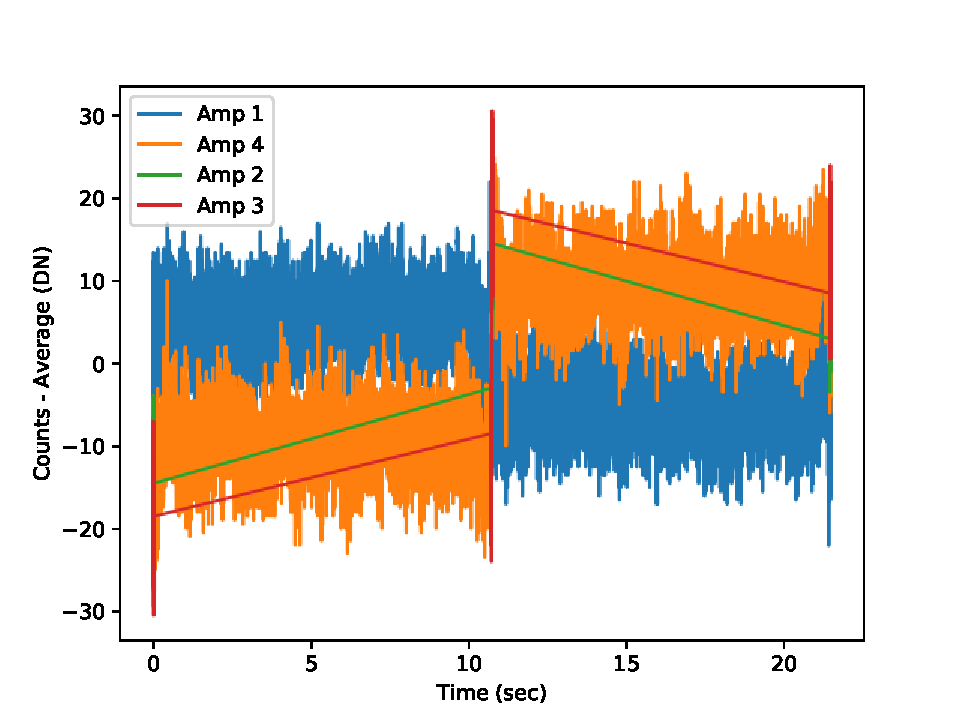
\includegraphics[width=.49\columnwidth]{allamps.pdf}
\includegraphics[width=.49\columnwidth]{allamps_long_dark.pdf}
\caption{Reference pixel time series for a two frame integration (Left) and a long dark integration of 108 frames (Right). Each of the plots show that the pre-amplifier resets between frames in an integration cause discontinuities in the reference signal. Amplifiers 1 and 4 track the time all through a frame with the side reference pixels, whereas amplifiers 2 and 3 in the middle only contain information on the bottom and top reference pixels at the beginning and ending of a frame.
The long dark exposure example of 108 integrations shows the behavior over long timescales.}\label{fig:ampResetDark}
\end{figure*}

\subsection{Amplifier Boundary Discontinuities}

NIRCam's STRIPE mode and full frame mode both employ 4 amplifiers to simultaneously read out or reset 4 pixels at once.
This simultaneous use of 4 amplifiers reduces the frame time by a factor of 4 and thus increases the brightness of objects that can be detected before saturation as well as increases the number of reads for a detector pixel before saturation to average readout noise.
Users have the option to select the 1 or 4 amplifiers with the ``No. of output channels'' in APT.
On the flip side, the four amplifiers will have different behaviors such as separate offsets in the bias level.
The differential biases between the amplifiers will show up as step function changes in the slope of the image at the amplifier boundaries (512, 1024 and 1536), as visible in Figure \ref{fig:ampOffsetsOtisGrismSlope} (top panel).
If a spectrum of a source is extracted without any vertical background extraction or reference pixel correction, the amplifier offsets cause sharp discontinuities in the summed spectrum.

Fortunately, the amplifier offsets are efficiently removed by reference pixels and background subtraction.
For example, subtracting the average reference pixel in each amplifier will reduce the offsets between amplifiers, shown in Figure \ref{fig:ampOffsetsOtisGrismSlope}, (second from top panel).
It should be noted, however, that there are gradients in the bias signal within each amplifier.
One could subtract the mean reference pixel in each column to reduce these gradients, shown in Figure \ref{fig:ampOffsetsOtisGrismSlope}, (third from top panel) but given that there are only 4 reference pixels at the bottom of each column, this introduces extra noise in the subtraction.
Instead, one can use the background region for each column ($\sim$80 pixels) to best remove gradients and the amplifier offsets.
Here, we find the average of all pixels from Y=0 to 15 and Y=190 to 256 in each column and subtract this value from the whole column.
This is repeated for all columns.
This background subtraction method will efficiently remove the pre-amplifier offsets to the level where amplifier discontinuities become smaller than the combined read and photon noise in the image.

\begin{figure*}[!hbtp]
\centering
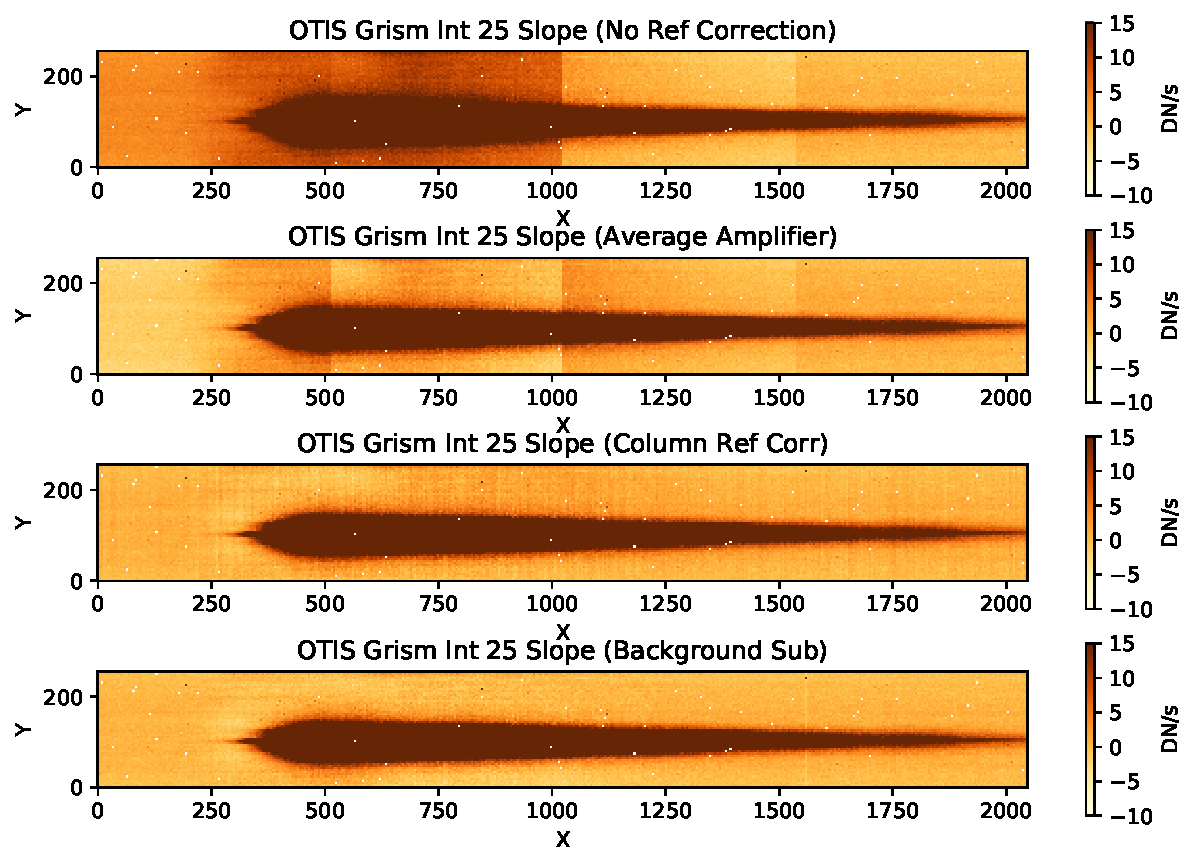
\includegraphics[width=.79\columnwidth]{amplifier_offsets_in_otis_lw_grism.pdf}
\caption{An example slope image from the LW OTIS Stability test.
{\it First Panel:} No reference pixel correction is applied, leaving offsets at the amplifier boundaries.
{\it Second Panel:} Averaging all the reference pixels within an amplifier and subtracting the result reduces the offsets between amplifiers but there are still noticeable boundaries at X= 512, 1024 and 1536.
{\it Third Panel:} Reference pixel correction using the 4 non-illuminated pixels in each column significantly reduces offsets between amplifiers, but introduces read noise to each column.
{\it Fourth Panel:} Background subtraction with the mean value of the pixels below Y=15 and above Y=190 eliminates offsets between amplifiers without introducing any substantial new noise source.
}\label{fig:ampOffsetsOtisGrismSlope}
\end{figure*}

\section{1/f Noise}
The readout circuitry for NIRCam and other JWST NIR instruments introduces correlated noise from pixel-to-pixel.
This is visible when examining the time series of pixels as they are read out within a frame in the order they are addressed.\footnote{See a diagram of the readout directions at \url{https://jwst-docs.stsci.edu/near-infrared-camera/nircam-instrumentation/nircam-detector-overview/nircam-detector-readout}}
The power spectrum of this pixel-by-pixel time series reveals high power at low frequencies that drops approximately like a 1/f power law in the power spectrum of the time series.
Figure \ref{fig:pixelTSeriesPSpec} shows the average Lomb Scargle periodogram from the readout amplifier over 108 dark frames.
To create the periodogram, the reference pixels are used to remove amplifier offsets between frames.
Next, the average of all frames is subtracted to remove the bias and all pixels that deviate by more than 80 DN from the average are masked to eliminate bad pixels.

Figure \ref{fig:pixelTSeriesPSpec} shows that the noise power drops nearly like 1/f from the lowest frequency in a frame to $\sim$1000 Hz, where the curve flattens out.
This indicates that the noise is closer to white noise, where each pixel's noise would be statistically independent from the others, at high frequencies.
The periodogram also shows many spikes at high frequency on top of the 1/f noise.
One of these prominent spikes occurs at the line reset time of 524 clock cycles, which is the time to read out all the pixels in a row for the amplifier and line overheads before moving to the next row.

The 1/f noise is compared to a simulated time series with the same robust standard deviation but with Gaussian white noise where each pixel is independent and identically distributed as a Gaussian.
It is clear from Figure \ref{fig:pixelTSeriesPSpec} that the 1/f noise and the periodic signatures significantly increase the power over uncorrelated white noise (green line) at low frequencies.
1/f rises above the white noise level at 70 cycles / 1400 Hz for amplifier 1 and the intersection ranges from 70 to 135 across the 4 amplifiers.
This power spectrum shows that the read noise is significantly correlated from pixel to pixel and this will affect both high precision spectroscopy and high precision photometry.

\begin{figure*}[!hbtp]
\centering
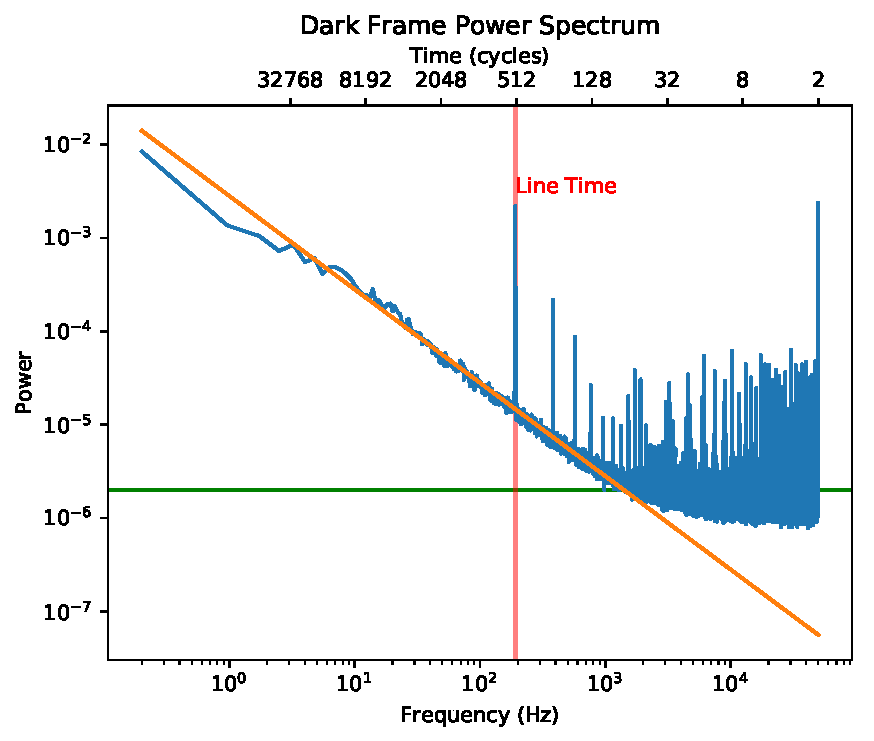
\includegraphics[width=.4\columnwidth]{avg_psd_amp_1.pdf}
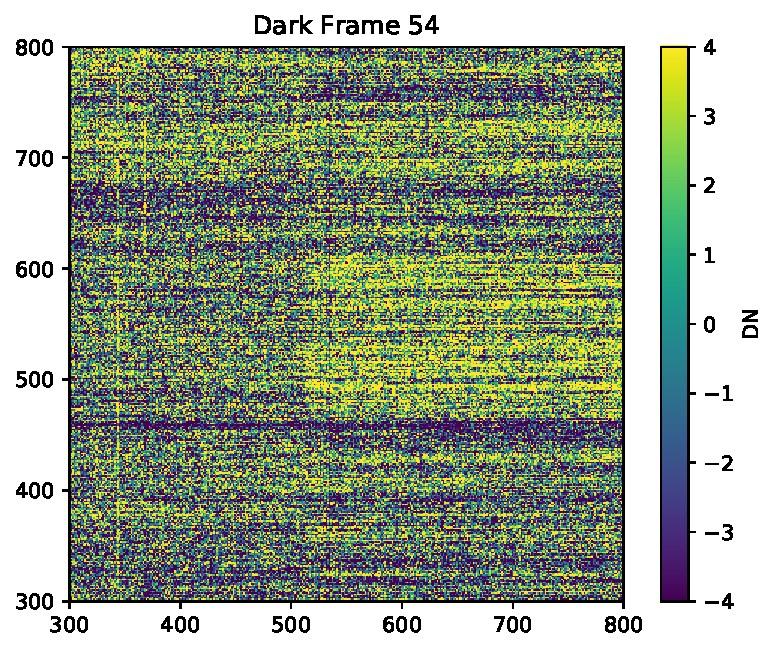
\includegraphics[width=.4\columnwidth]{preamp_removed_grp_54.pdf}
\caption{{\it Left:} The average Lomb-Scargle periodogram from Amplifier 1's time series over 108 groups.
The noise in the spectrum is close to a 1/f power law (orange line) from 10 to 1000 Hz.
Above 1000 Hz, it is closer to white noise (green line) with spikes at specific frequencies.
{\it Right:} This 1/f noise introduced in the readout circuit causes prominent correlated noise along the fast-read direction (horizontal) on a dark frame.
The amplifier offsets have been removed, but the 1/f noise from these adjacent amplifiers (separated at X=512) shows different behavior.
}\label{fig:pixelTSeriesPSpec}
\end{figure*}

The 1/f noise can be reduced by subtracting reference pixels and/or active pixels over the aperture of interest.
As the power spectrum shows, the 1/f noise begins to contribute significantly for frequencies below 1000 Hz (i.e., timescales longer than 100 cycles, where a cycle is the 10$\mu$s time to address a pixel).
Ideally, source apertures would be less than 100 pixels wide so that background subtraction along rows will remove the 1/f noise but this is impossible for grism spectra dispersed along the rows.
NIRCam has a ``GRISMC" grism that will disperse along the column direction but this mode would not work with horizontal stripe subarrays and would therefore saturate on bright targets with $K \lesssim 5.5$.
For this reason, the ``GRISMC'' is not currently available for time series observations.

\subsection{Long Darks}\label{sec:longDarks}

It is instructive to look at dark frames to isolate the contributions of the read-out electronics, including the SIDECAR ASIC, and how much they contribute to the error budget.
The dark frames do not have issues with the photometric stability of illumination lamps, which is a persistent challenge with ground-based tests.
They also do not contain photon noise in the background, which can make electronic noise sources harder to see.
We study here the contributions from read noise, including the 1/f noise from the electronics.
This experiment with dark frames does not test subtle changes in behavior of the electronic read noise under illumination, such as crosstalk where pixels that have no direct flux from a source in an image correlate with other regions of the detector with high flux rates.

A standard long dark exposure used for detector characterization is a single integration that is 108 groups of 1 frame each (RAPID mode).
The detectors are read in full frame mode so that each frame is 10.73677~s in duration with 4 output amplifiers in use, thus the total time for the exposure is 19.3 min.
We use one of these long dark integrations to create simulated time series as if it were observing many consecutive integrations in full frame mode.
The long darks are broken into 54 sequential pairs of images that are subtracted from each other (integration 1 minus integration 0, 3 minus 2, 5 minus 4 etc. in a zero-based counting scheme).
We also re-label the times to include the reset time that would normally occur after each integration, so the Figure \ref{fig:longDarkPhot} shows an example dark read pair from frame 55 minus frame 54.
In the raw data, there are 4 prominent vertical stripes that are 512 pixels wide and 2048 pixels tall due to offsets in the read-out amplifiers.
These amplifier offsets are caused by drifts in the reference voltage that are reset once per frame and vary from amplifier to amplifier.
Additionally, there are obvious correlations along the fast-read (X) direction due to 1/f noise that appear as horizontal stripes in the image.

The ramps-to-slope pipeline \texttt{ncdhas} or the STScI JWST pipeline will apply reference pixel correction, bad pixels masks and non-linearity correction before fitting the groups up the ramp to a line.
In this work, we use \texttt{ncdhas}.
As seen in Figure \ref{fig:longDarkPhot}, reference pixels can be used to reduce the large offsets between amplifiers.
The reference pixels are comprised of a 4 pixel boundary along the edges of the detector, which are not connected to detector photodiodes and can therefore be used to measure common-mode electronic noise without being affected by photon counting noise.
The reference pixels are most useful for subtracting the offsets between amplifiers because there are 8 rows of 512 pixels or a total of 4096 reference pixels to average for each amplifier at the bottom and top of the arrays.
There are an additional 4 columns on the left and right side boundaries (8176 pixels) that can be used to further correct the left and right amplifier offests.
However, the 1/f noise that correlates along the fast-read (X) direction is more difficult to remove with reference pixels.
Only 4 pixels on the left and 4 pixels on the right side may be used to subtract the 1/f noise in a given row and the 4 amplifiers can exhibit different 1/f noise. 
Therefore, significant residuals remain along the fast-read (X) direction in the reference-corrected read pair shown in Figure \ref{fig:longDarkPhot}.
These side reference pixels also cannot correct for read noise correlations that happen on shorter length scales than 512 pixels (5 ms).

\begin{figure*}[!hbtp]
\centering
\includegraphics[width=.32\columnwidth]{ap_labels_dark_NRCALONG-DARK-7235074213_1.pdf}
\includegraphics[width=.32\columnwidth]{ap_labels_darkRed_NRCALONG-DARK-7235074213_1.pdf}
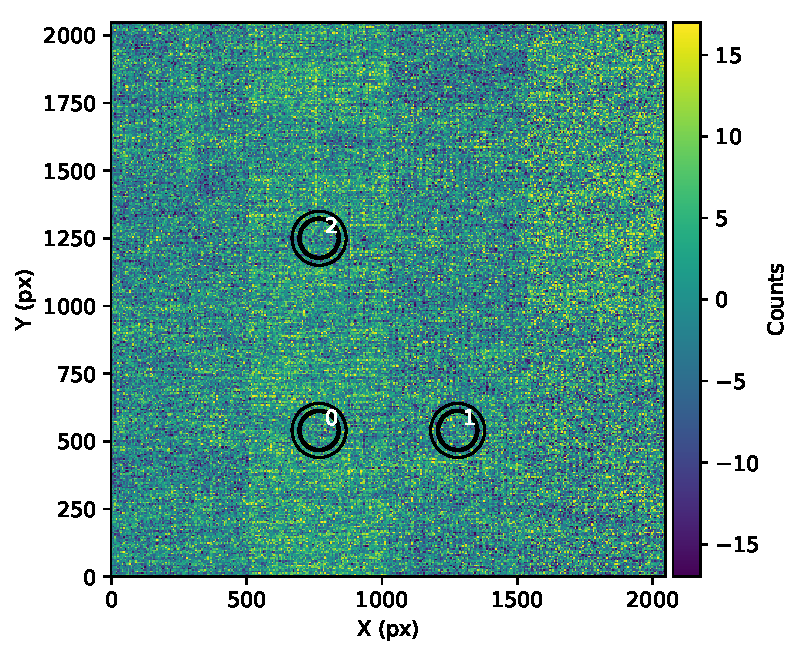
\includegraphics[width=.32\columnwidth]{ap_labels_row_by_row_group_sub_aps_1_NRCALONG-DARK-7235074213_1.pdf}
\includegraphics[width=.32\columnwidth]{long_dark_dark.pdf}
\includegraphics[width=.32\columnwidth]{long_dark_darkRed.pdf}
\includegraphics[width=.32\columnwidth]{long_dark_darkRedRowSub.pdf}
\caption{Time series of a 70 pixel radius photometric aperture obtained during a long dark exposure for detector ALONG=A5. The long dark exposure of 108 frames is used to construct 54 pairs of reads that are subtracted, in analogy with a series of integrations.
{\it Top:} Example read pair subtraction with an overlay of the apertures for 3 different reduction steps from ``Raw" data using no reference pixel correction, reference pixel-correction that uses the top, bottom and side reference pixels and finally a method using a row-by-row median subtraction.
{\it Bottom} The time series for each circular aperture with background subtraction using a circular annulus.
Both the pre-amplifier offsets and row-by-row 1/f subtractions are important to reduce the effective read noise in the aperture.
}\label{fig:longDarkPhot}
\end{figure*}

\subsection{Photometric Aperture}\label{sec:photApertureDark}

Exoplanet transit measurements are dependent on the photometric stability within an aperture or spectrum.
We therefore perform aperture photometry on the dark frame as if it were a weak lens image with a 70 pixel radius circular source aperture and a 75 to 100 pixel background annulus illustrated in Figure \ref{fig:longDarkPhot}.
%Also, Figure \ref{fig:WLP8PSF} shows an example weak lens PSF with this aperture.
The background subtraction will largely remove the offsets affecting the whole 512$\times$2048 amplifier.
However, the correlated 1/f noise along the X direction will not be subtracted efficiently by an annulus.
Instead, a row-by-row line fit to the background can be more effective.

For a read pair subtraction, the ``CDS'' (correlated double sample) read noise is 13.3 e$^-$ or 7.2 DN for the A5 detector studied here.
If we assume each pixel's read noise is uncorrelated with its neighbors, the total noise within the source aperture is then $\sqrt{N_{px}} \times RN $ where $N_{px}$ is the number of pixels and $RN$ is the read noise of a single pixel.
If we also assume that the background pixels are uncorrelated with each other and the source pixels, then the total noise in background-subtracted photometry is 1310 DN.

This theoretical read noise is smaller than the photon noise expected inside an aperture during photometric stability time series applications.
The number of DN collected within a 70 pixel radius aperture for a weak lens plus 8 waves (WLP8) image in our CV3 detector stability test with 2 groups in RAPID, equivalent to a correlated double sample (CDS), was $S_{tot}=3.9\times 10^7$ DN during the integration.
The peak pixel counts in this integration were 30,000 DN or about 60\% well depth for the A1 detector.
The Poisson shot noise for photons is $N_{phot} = \sqrt{S_{tot}} / \sqrt{G} = 4,400$ DN, where $G$ is the gain ($G \approx 2.0$ for the short wave (SW) detectors).
In terms of fractional noise, the photon shot noise should be 113 ppm and the read noise should be 33 ppm.
Therefore, the read noise is expected to be about 1/4 the shot noise for 2 group RAPID read mode (i.e., CDS).
When averaging together 111 full frames over 60 minutes (an order-of-magnitude transit duration for most planets), the photon noise would contribute 11 ppm and the read noise would contribute 3 ppm.

In our experimental time series, however, the standard deviation in the time series in these 3 apertures is 22,000 to 25,000 DN (without any attempt to correct for amplifier offsets or 1/f noise using reference pixels or otherwise).
If uncorrected, this extra read noise will contribute 560 to 630 ppm to the time series per read pair!
This read noise would be $\sim$5$\times$ the $\sim$113 ppm photon noise.
However, there are ways to significantly reduce the pre-amplifier offsets and 1/f noise.

\begin{deluxetable*}{c|cc|cc}[b!]
\tablecaption{Summary of Noise Sources in Long Dark Test}
\tabletypesize{\footnotesize}
%\tablecolumns{7}
%\tablenum{2}
\tablewidth{0pt}
\tablehead{
\colhead{Aperture} &
\multicolumn{2}{c}{WLP8} &
\multicolumn{2}{c}{Grism 0.17 $\mu$m bin}\\
\colhead{Noise Description} &
\colhead{$\sigma$} &
\colhead{$\sigma$} &
\colhead{$\sigma$} &
\colhead{$\sigma$} \\
\colhead{} &
\colhead{DN} &
\colhead{ppm} &
\colhead{DN} &
\colhead{ppm}\\}
\startdata
Ideal Photon Noise & 4,400 & 113 & 1,430 & 388 \\
Ideal Uncorrelated Read Noise & 1,300 & 33 & 350 & 94 \\
\hline
Measured Read Noise with amplifier offsets (no correction) & 23,500 & 600 & 80,930 & 21,900  \\
Measured Read Noise (reference pixel correction) & 10,800 & 280 & 9,900 & 2,680 \\
Measured Read Noise (reference channel subtraction) & 9,700 & 250 & & \\
Measured Read Noise (row-by-row subtraction) & 6,000 & 150 & 3,860 & 1044 \\
Measured Read Noise (20 Component PCA subtraction) & 5,400 & 140 & & \\
Measured Read Noise (smoothed 161 px kernel interpolating over aperture) & 3,300 & 85 & & \\
Measured Read Noise (5 Component PCA on each amplifier) & 3,200 & 81 & & \\
Measured Read Noise (row-by-row amp-by-amp mean subtraction) & 2,900 & 75 & & \\
Measured Read Noise (smoothed 40 px kernel on top of aperture) & 900 & 23 & & \\
Measured Read Noise (variance-weighted summation)	& & & 3,060 & 830 \\
Measured Read Noise (covariance-weighted summation)	& & & 850 & 230 \\
\enddata
\tablecomments{The theoretical and measured noise sources in one integration for a weak lens +8 waves and grism time series.
The ppm units are assuming a peak 60\% well depth or 3.9$\times 10^7$ DN during an integration for the weak lens PSF and 3.7$\times 10^6$ DN during and integration for the grism PSF.
The noise is reported for the the aperture/spectral extraction (in DN) or relative to the photon signal (in ppm).
The integration is assumed to be a bright source with 2 groups of 1 integration each up the ramp (i.e., CDS).
For the grism, statistics are shown for a representative 0.17~$\mu$m wide wavelength bin centered on 3.34~$\mu$m.}
\label{tab:noiseSummary1overf}
\end{deluxetable*}

These large correlations in read noise can be reduced with the reference pixels, which are designed to track electronic noise without the presence of background photon noise.
We use the \texttt{ncdhas} pipeline to apply reference pixel correction, which dramatically reduces the amplifier offsets and also reduces 1/f noise correlations along the fast read (X) direction.
The time series for the 3 apertures considered drops to levels from 10,000 DN to 11,500 DN (depending on detector), but still falls short of the expectation of 1,310 DN if the read noise is uncorrelated.

\subsubsection{Row-by-Row Subtraction}\label{sec:photRowByRow}

Since these 8 reference pixels in each row are not sufficient to remove all 1/f noise in each row, we perform another correction step:
We find the median of each group up the ramp along the fast read (X) direction and subtract this from every row.
This amounts to a row-by-row background subtraction.

In the latter case, the standard deviation of the time series drops to 6000 DN, but is still larger than the expectation of 1310 DN if all noise were uncorrelated.
The A3 detector used for weak lens photometry has reduced 1/f noise.
%The standard deviation of the raw time series is 15,000 compared with the 22,000 from the A5 (ALONG) detector.

\subsubsection{Mean Row by Amplifier}\label{sec:indAmpAvg}
A slight modification to the above strategy is to average each amplifier individually.
This takes care of any differences between amplifiers.
This individual amplifier dramatically decreases the errors.
The standard deviations of the background-subtracted photometry range from 2,540 to 3,300 DN or 65 to 85 ppm across detectors.
Therefore, this simple approach can dramatically decrease the 1/f noise to well below the photon limit.
This is possible for weak lens photometry but not grism spectroscopy when dispersed parallel to detector rows (the fast-read direction).

\subsubsection{Smoothed Kernel Subtraction}\label{sec:smoothKernelSub}

We also consider more sophisticated ways to reduce read noise than the median row subtraction discussed in Section~\ref{sec:photRowByRow}.
We start by applying a smoothing kernel to each group (1 read for RAPID mode) up the ramp of the raw data.
The kernel is a uniform normalized kernel 1 pixel in height and 40 pixels along a row.
This enables subtraction of 1/f noise that has length scales shorter than the line time (i.e., timescales shorter than 512 clock cycles or 5 ms), which the median subtraction cannot remove.

This smoothing kernel makes a dramatic improvement to the final weak lens aperture time series, as shown in Figure \ref{fig:longDarkWithRowKernel}.
The standard deviation in the time series drops from the best previous method (row and column median subtraction) by a factor of nearly 10!
For the row and column median subtraction applied to the red files, the standard deviation was 6,150, 5,600 and 6,600 DN for apertures 0, 1 and 2. For the same apertures, the standard deviation in the time series drops to 650, 890 and 570 DN.

\begin{figure*}[!hbtp]
\centering
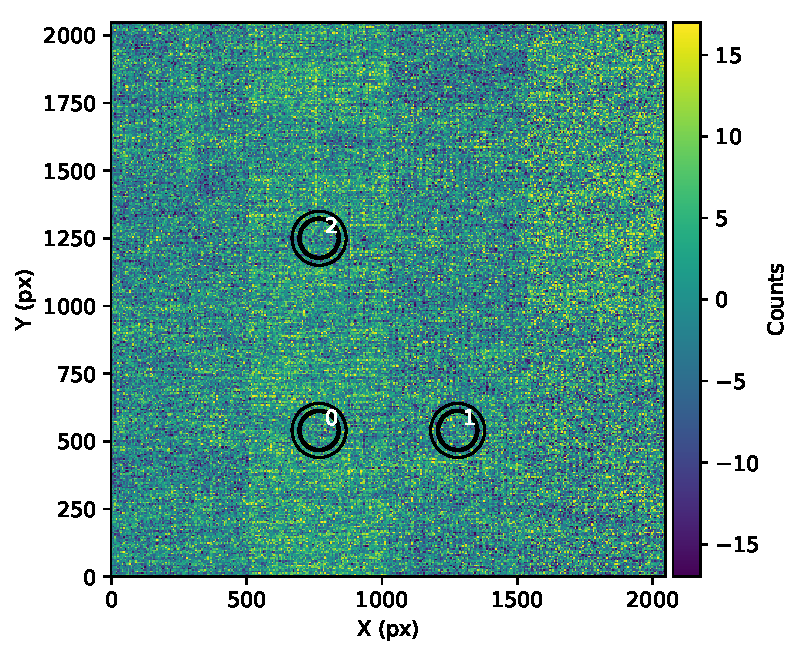
\includegraphics[width=.37\columnwidth]{ap_labels_row_by_row_group_sub_aps_1_NRCALONG-DARK-7235074213_1}
\includegraphics[width=.37\columnwidth]{ap_labels_darkRedsmoothedRowKernel_NRCALONG-DARK-7235074213_1.pdf}
\includegraphics[width=.37\columnwidth]{zoom_long_dark_row_by_row_group_sub.pdf}
\includegraphics[width=.37\columnwidth]{zoom_long_dark_darkRedsmoothedRowKernel.pdf}
\caption{The same apertures as Figure \ref{fig:longDarkPhot}, but with subtraction by a smoothed image where a 40 pixel wide and 1 pixel tall averaging kernel was applied along the fast read direction of every group.
Subtraction by the smoothed image has a dramatic effect on reducing correlated 1/f read noise from $\sim$6,000 DN to $\sim$700 DN in the aperture.
}\label{fig:longDarkWithRowKernel}
\end{figure*}

The dramatic difference from the smoothing kernel is beyond what is possible for a real source.
This is because the 40 pixel wide kernel was applied all the way through the source aperture, which would subtract and distort any signal from a star/planet source.
In reality, the kernel should be wider than the source aperture diameter and interpolate through the source points.
Note that this experiment would result in perfect subtraction (0 ppm noise) if the kernel was only 1 pixel wide.
We repeated the experiment with a 161 pixel wide kernel and masked bad pixels and the source pixels.
We use the \texttt{astropy.convolution.convolve()} routine, which calculates a convolution of the kernel by the image.
\texttt{astropy.convolution.convolve()} ignores all NaN values in the mask and renormalizes the kernel by the sum of the remaining kernel points.
This efficiently interpolates over bad pixels and can also interpolate over the source aperture.
Our smoothing kernel is a flat boxcar normalized to 1.0.
This more realistic kernel results in higher noise because of its larger window size and because it interpolates over the aperture points.
The resulting time series has a standard deviation of 2800 DN to 3700 ppm.
This is still larger than the 1,300 DN expectation for uncorrelated read noise, but is below the ideal photon noise limit when integrations reach 60\% well depth.

\begin{figure*}[!hbtp]
\centering
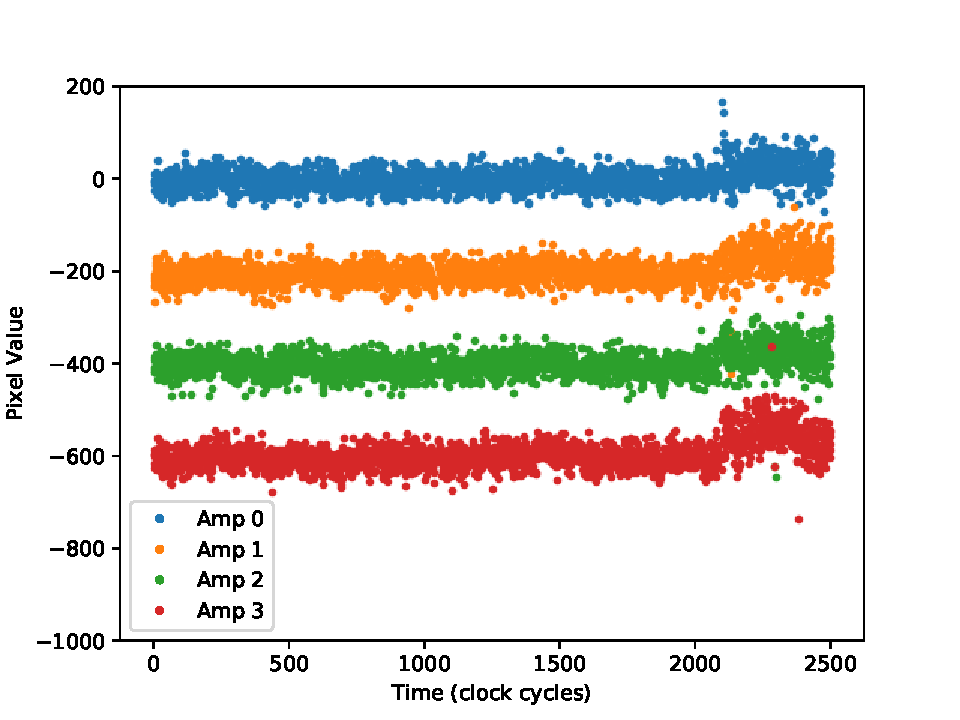
\includegraphics[width=.32\columnwidth]{pixeltime_series_0.pdf}
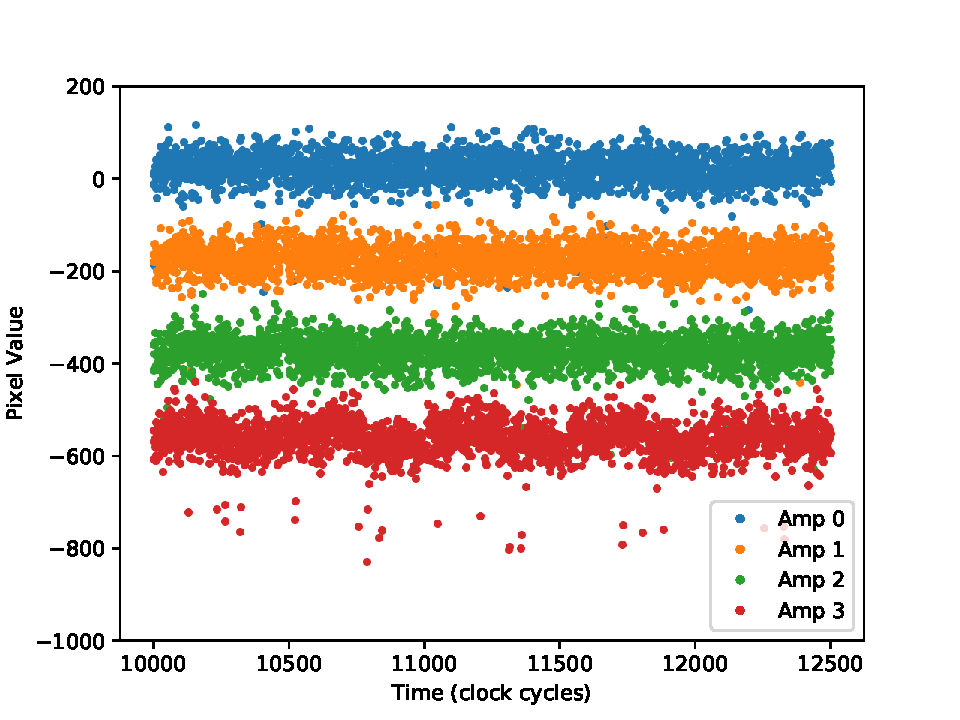
\includegraphics[width=.32\columnwidth]{pixeltime_series_1.pdf}
%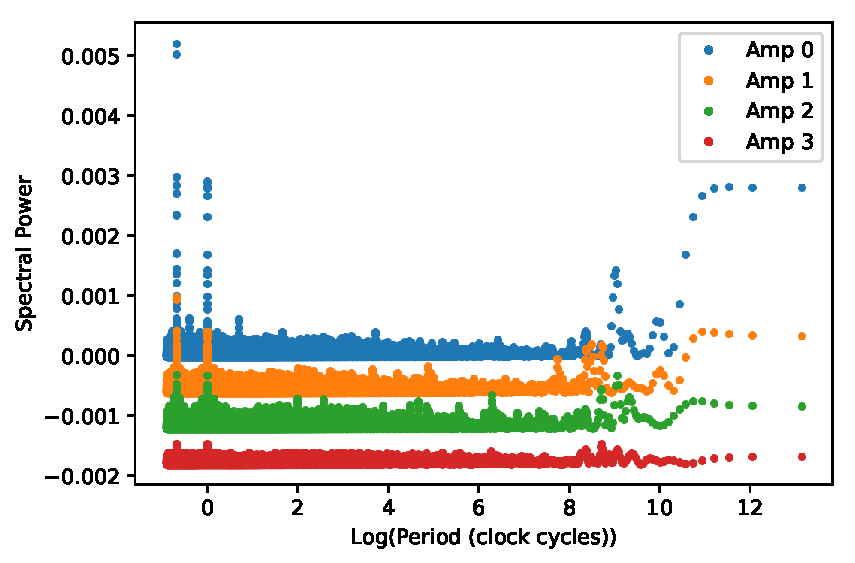
\includegraphics[width=.32\columnwidth]{all_amp_periodograms.pdf}
\caption{The time series for all 4 amplifiers share common-mode behaviors for some intervals but not always (left and right plots).
This is visible in a short segment of the time series of all pixels for an example group up-the-ramp 53 in a dark ramp where the bias has already been subtracted.
The pixels in each time series are smoothed with a 51 pixel-wide median filter to show the low frequency noise.
The left panel shows the a time near the beginning of a frame, where amplifiers 1 and 2 share some common-mode read noise.
The right panel shows another part of the time series where amplifiers 1 and 2 have more disparate noise signatures.
}\label{fig:darkPixelTimeSeries}
\end{figure*}

\subsubsection{Reference Channel Subtraction}
We note that the 4 channels can sometimes exhibit the same 1/f correlation behavior, as shown in Figure \ref{fig:darkPixelTimeSeries}.
Another option to remove 1/f noise is to subtract the illuminated amplifier with a target in it by un-illuminated channels.
We subtract an amplifier 0's time series from all amplifiers.
Of course, this means that this amplifier is perfectly subtracted and no noise or signal remains in this 1/4 of the image.
The subtraction step should increase the read noise on an individual pixel by $\sim \sqrt{2}$ because the errors from the subtracted pixel should add in quadrature to the original pixels.
This increase in read noise on a per-pixel level might be acceptable if it decreases the correlated errors along the rows.
On the other hand, if the each amplifier exhibits its own individual correlated noise behavior, the reference amplifier will fail to subtract out all correlated noise and may introduce more noise.

The net effect of this method is to increase the noise over a row-by-row median subtraction.
The standard deviations in the time series range from 8,500 DN to 10,800 DN for this reference amplifier method as opposed to the 5,500 DN to 6,600 DN for a row-by-row median.
This means the correlations within an amplifier are not efficiently subtracted and may be propagated to the remaining amplifiers.

\subsubsection{PCA Correction}

\begin{figure*}[!hbtp]
\centering
\includegraphics[width=.4\columnwidth]{pca_dark_amp_all_extra_bias_sub_grp_54.pdf}
\includegraphics[width=.4\columnwidth]{pca_dark_amp_all_extra_bias_sub_grp_55.pdf}
\caption{The first 10 principal component eigenvectors identified from group 54 (left) and group 55 (right).
Pre-amplifier reset values are seen in the first principal component, and change from one group (one read in RAPID) to another.
These are residual values are not fully subtracted by reference pixels.
The principal components generally increase in frequency with principal component number.
In other words, the highest frequency principal components explain the least amount of the variance as would be expected for 1/f noise.
}\label{fig:pcaEigenvectors}
\end{figure*}

Another approach to treating the 1/f noise is dimensionality reduction with principal component analysis (PCA).
Here, we assume that the counts for each pixel along a column is a random variable that can be correlated with pixels in other columns.
Each row represents a different noise iteration.
First, we apply reference pixel correction to remove the pre-amplifier resets.
Next, we calculate the mean value of each pixel in the 108 group stack and subtract all groups by this mean image.
This removes all bias levels and focuses on the time variability of the pixels.
Here, we assume the dark current is negligible.
Next, we mask all bad pixels by setting all pixels with an absolute value larger than 200 DN and replace them with 0 DN to remove bad pixels that can drive the principal components.
The first 10 principal components are plotted in Figure \ref{fig:pcaEigenvectors} for two example groups (54 and 55).

The first 10 principal components explain 14\% of the total variance in each group up the ramp.
The principal components from one group to another are different, but the ordering of these components generally follows a pattern of increasing frequency with higher order principal components (smaller eigenvalues).
This is expected for 1/f noise where the lowest frequencies have most of the power.
Since the first principal components are different from one group to another, we calculated the principal components for each group independently.
We then create a noise model image which is the matrix multiplication of the eigenvectors by the principal components for 10 components.
This model is subtracted from each group to create a 1/f-corrected image.

The PCA subtraction is applied to each group up-the-ramp and then these groups are subtracted in pairs to create a time series.
We use 20 principal components as a starting point for this method.
The final time series has a measured standard deviation of 5,300 to 5,500 DN within the background-subtracted aperture.
This is comparable to the row and column subtraction standard deviation of 5,500 to 6,500 DN.
Adding 10 more principal components for a total of 20 eigenvectors only reduces the time series noise to 5,100 to 5,400 for the 3 apertures.

In another approach, we treat each amplifier separately so that the principal components are calculated independently.
This approach means that a noise signature in 3 amplifiers but not the fourth does not propagate to fourth amplifier when subtracting the PCA-based model.
This individual-amplifier model has four times the number of variables as the combined PCA approach, so we fit with only the first 5 principal components in each amplifier.
The resulting eigenvectors are shown in Figure \ref{fig:pcaEigenvectorsIndAmp}.

If we treat each amplifier separately, the PCA model is more effective in reducing 1/f noise.
We begin by keeping 5 principal components within each amplifier and subtracting these from each amplifier separately.
The resulting standard deviation of the time series is 2,500 to 3,820 DN.
This improvement is beyond what is possible on a real source because the principal components include pixels over the source aperture.
To simulate a real photometry scenario, it is necessary to interpolate over the source aperture points as done in Section \ref{sec:smoothKernelSub} for the smoothing kernel.
However, we stop the PCA at this point because it does not do as well as the simple row-by-row amplifier-by-amplifier mean subtraction performed in Section~\ref{sec:indAmpAvg}.

\begin{figure*}[!hbtp]
\centering
\includegraphics[width=.4\columnwidth]{pca_dark_ind_amp_grp_54_extra_bias_sub.pdf}
\includegraphics[width=.4\columnwidth]{pca_dark_ind_amp_grp_55_extra_bias_sub.pdf}
\caption{The first 5 principal component eigenvectors identified from group 54 (left) and group 55 (right) where each amplifier has been analyzed independently.
The amplifier boundaries are demarcated by solid vertical lines.
}\label{fig:pcaEigenvectorsIndAmp}
\end{figure*}

\begin{figure*}[!hbtp]
\centering
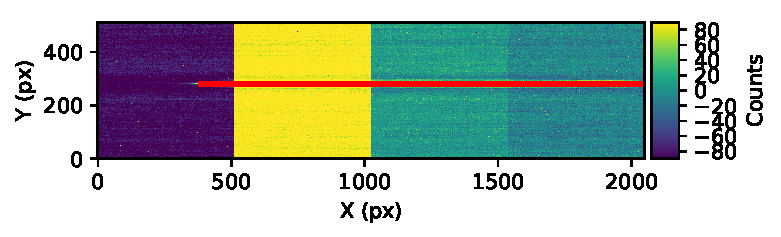
\includegraphics[width=.32\columnwidth]{spec_aps_pairwiseSubNoRed_otisLongDarkSimGrism.pdf}
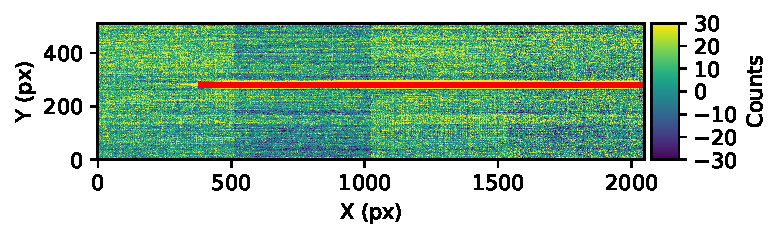
\includegraphics[width=.32\columnwidth]{spec_aps_pairwiseSubRed_covWeights_otisLongDarkSimGrism.pdf}
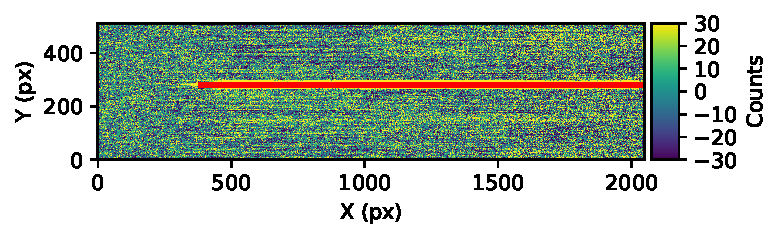
\includegraphics[width=.32\columnwidth]{spec_aps_pairwiseSub_backsub_otisLongDarkSimGrism.pdf}
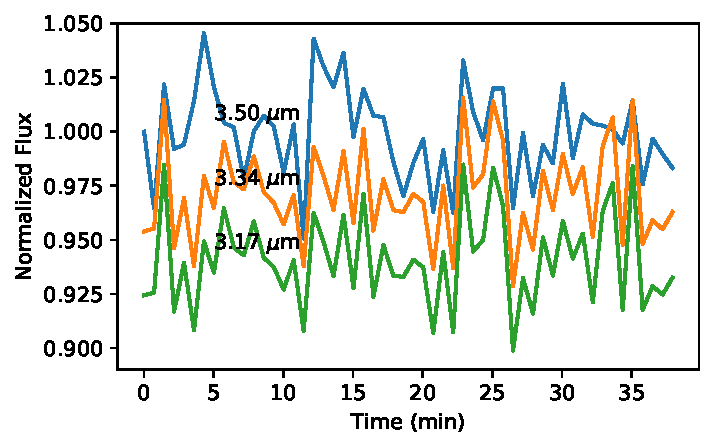
\includegraphics[width=.32\columnwidth]{tser_pairwiseSub_noRed01.pdf}
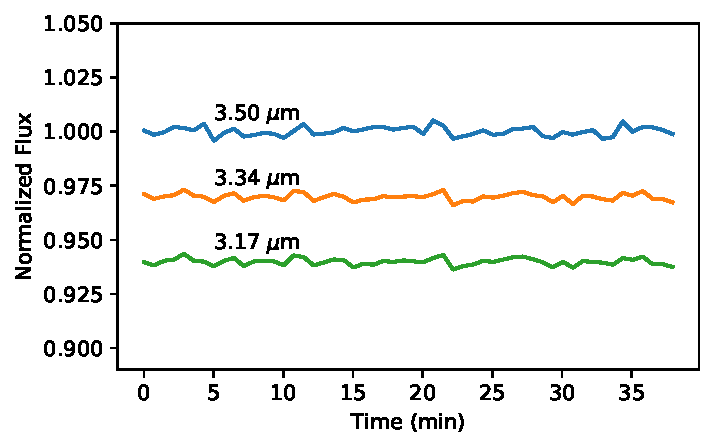
\includegraphics[width=.32\columnwidth]{tser_pairwiseSubRed.pdf}
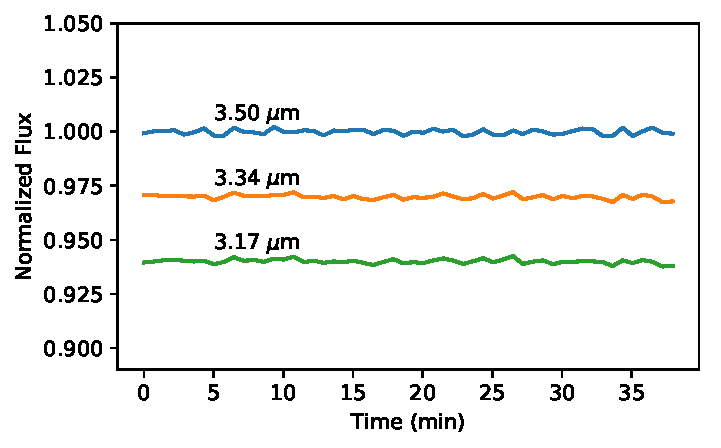
\includegraphics[width=.32\columnwidth]{tser_pairwiseSubRed_backsub.pdf}
\caption{{\it Top Row:} The read pairs have significant pre-amp offsets and 1/f noise (left), which are reduced by reference pixels (middle) and column-by-column, row-by-row subtraction (right).
The spectrum (outlined in red aperture box) is dispersed along the fast read (horizontal) direction, so it is particularly susceptible to 1/f noise.
{\it Bottom Row:} The standard deviation of the time series dramatically decreases from 21,900 ppm to 2,680 ppm with reference pixels and 1044 ppm with column-by-column, row-by-row subtraction for the 3.34 $\mu$m bin.
Here, the simulated grism image for an F322W2 filter spans 3 amplifier channels (512 pixels wide) and part of the leftmost amplifier, so only reference pixels and horizontal pixels with X $<$ 300 can be used to reduce the 1/f noise.
}\label{fig:longDarkGrism}
\end{figure*}

\subsection{Grism Extraction}\label{sec:GrismDarkExtraction}

The NIRCam grism time series are particularly susceptible to 1/f noise because the dispersion direction is parallel to the detector's fast-read direction.
This is visible in Figure \ref{fig:longDarkGrism} where the grism apertures (in red) are parallel to the 1/f noise correlations.
The background subtraction along the spatial direction (vertically) will efficiently remove pre-amplifier offsets from frame to frame and amplifier to amplifier.
However, there are only limited background regions along the horizontal direction available to subtract out 1/f noise.
This will result in increased noise on the right three amplifiers for the F322W2 filter (2.4 to 4.0 $\mu$m over $\sim$1600 px) and the left two amplifiers for the F444W filter (3.9 to 5.0 $\mu$m over $\sim$2100 px).

%, on the right three amplifiers for the F322W2 filter (2.4 to 4.0 $\mu$m over $\sim$1600 px) and the left two amplifiers for F444W filter (3.9 to 5.0 $\mu$m over $\sim$2100 px).

We give some illustrative numbers for a 0.165 $\mu$m wide bin of a grism spectrum centered on 3.34 $\mu$m as listed in Table \ref{tab:noiseSummary1overf}.
Without reference pixel subtraction, the grism apertures have standard deviations of 80,930 DN.
Reference pixel subtraction drops this value to 9,900 DN and row-by-row subtraction drops it to 3,860 DN.
For a well depth of 60\%, there are $3.7 \times 10^6$ DN of source counts in the 0.17 $\mu$m bin, which amounts to a photon error of 1,430 DN assuming a gain of 1.8.
Therefore, 1/f noise can potentially dominate the error budget for broadband grism time series.
Expressed in ppm, the read noise after processing with row-by-row subtraction is 1,044 ppm as compared to a photon noise of 390 ppm for a CDS subtraction (2 groups in ramp).

Given the high 1/f read noise, it is important to maximize the number of samples up the ramp.
The read noise averages down like $\sqrt{N}$ statistics (i.e., each read can be assumed independent and identically distributed).
Therefore, for the example bin size of 0.17~$\mu$m, there should be at least 7 reads to average per integration.
For RAPID and BRIGHT1 modes, there should therefore be 7 groups and for BRIGHT2, there should be at least 4 groups (of 2 frames each).
This would make the photon noise about equal to the read noise but ideally the read noise should be a small fraction of the photon noise.

Given the high level of correlation between pixels, another way to reduce 1/f noise is with a small aperture.
For example, a 13 pixel wide aperture results in measured read noise of 1044 ppm for the same 0.17$\mu$m wide bin centered at 3.34$\mu$m whereas a 3 pixel wide aperture results in a measured read noise of 290 ppm, which is below the expected photon noise.
However, this will sacrifice photons, so there must be a balance between reducing 1/f noise while capturing as many photons as possible.
Therefore, a weighting scheme expanded from optimal extraction \citep{horne1986optimalE} is preferred.

\subsubsection{Optimally Co-Variance Weighted Flux}\label{sec:optimalCovWeights}

Here, we provide a modification to the optimal extraction formula from \citet{horne1986optimalE}, that uses the covariance matrix of correlated pixels.
The goal is to find a scheme that estimates the total flux by summing the value in each pixel $j$.
We start by calculating a profile function $P_j$ that describes the fraction of the total flux in pixel $j$.
The profile is normalized so that
\begin{equation*}
\sum_{j=1}^{m} P_j = 1.
\end{equation*}
Any pixel can be used to estimate the total flux $f_i$ by dividing by the profile.
\begin{equation*}
f_j = \frac{S_j}{P_j},
\end{equation*}
where $S_j$ is the background-subtracted flux.
Therefore, the flux total is a weighted average of each pixel's estimate of the total flux $f_j$.
The goal becomes a weighting scheme to determine which weights $w_j$ minimize the variance in the total background estimate:
\begin{equation*}
f_{opt} = \frac{\sum_{j=1}^{m} w_j \frac{S_j}{P_j}}{\sum_{j=1}^{m} w_j}.
\end{equation*}

If one assumes that all pixels are independent thereby having zero correlation, the optimal weights (ones that minimize the variance in $f_{opt}$) are
\begin{equation}\label{eq:varianceweights}
w_j = \frac{1}{\mathrm{Var}(\frac{S_j}{P_j})} = \frac{1}{\frac{1}{P_j^2} \mathrm{Var}(S_j)} = \frac{P_j^2}{V_j},
\end{equation}
where Var() is the variance or the expectation of the squared deviation from the mean and $V_j =$Var$(S_j$) \citep{horne1986optimalE}.
Exoplanet observations, where high signal to noise is needed to remove the planet from star signal, are generally in the foreground limit (where the variance is approximately equal to the number of photons).
In this case, both the profile $P_j$ and variance $V_j$ will be proportional to the number of photons $N_{phot}$, so the pre-multiplier of the flux becomes:           
\begin{equation*}
\frac{w_j}{P_j} \approx \frac{N_{phot}^2}{N_{phot} N_{phot}} = 1.0.
\end{equation*}
Therefore, using this traditional formula will provide little difference with straight summation,
\begin{equation}\label{eq:StraightSummation}
f_{sum} = \sum_{j=1}^{m} S_j.
\end{equation} 

However, in the presence of noise correlations, the formulae become modified.
The optimal weights for correlated data are the sums of the inverse covariance matrix along one dimension  \citep{schmelling1995averagingCorrelatedData},
\begin{equation}\label{eq:covarianceweights}
w_j = \sum_{i=0}^{m} C_{ij}^{-1},
\end{equation}
where $C_{ij}$ is the covariance (Cov()) of the variable $S_i/P_i$ with $S_j/P_j$,
\begin{equation}
C_{ij} = \mathrm{Cov}\left(\frac{S_i}{P_i},\frac{S_j}{P_j}\right) = \frac{1}{P_i P_j} \mathrm{Cov}(S_i,S_j).
\end{equation}

The variance in the flux is
\begin{equation}
\mathrm{Var}(f_{opt}) = \frac{1}{\sum_{j=1}^m w_j}.
\end{equation}

In Section \ref{sec:empCovarianceMatrix}, we compare the results of straight summation (Equation \ref{eq:StraightSummation}), variance weighting (Equation \ref{eq:varianceweights}) and covariance weighting (Equation \ref{eq:covarianceweights}).
%Simply variance weighting the spectra by the read and photon noise does not provide heavy enough weights.
%If we assume the read noise is perfectly correlated along the spectral direction and uncorrelated along the spatial direction, then equation \ref{eq:covarianceweights} becomes
%\begin{equation}
%w_j = \frac{P_j}{N_{ph} + N_{px} \sigma_R^2},
%\end{equation}
%where $N_{px}$ is the number of spectral pixels that will be binned and $\sigma_R$ is the read noise per pixel.
%Thus, for large values of $N_{px}$ (up to 512 for an amplifier), the $\sigma_R \approx 14e^-$ of read noise per pixel, can compound to 100,400 e$^-$ and the weighting approaches
%\begin{equation}
%w_j \propto P_j.
%\end{equation}
%
%Profile weighting should therefore lower the error on wavelength-binned time series.
%For the grism aperture experiment, we find that profile weighting gives a measured read noise of 355 ppm.
%Thus, profile weighting still does not reduce the standard deviation over an extraction aperture that is just 1 pixel wide at the peak grism flux.
%We show the real covariance matrix in Section \ref{sec:empCovarianceMatrix}.
\begin{figure}[!hbtp]
\centering
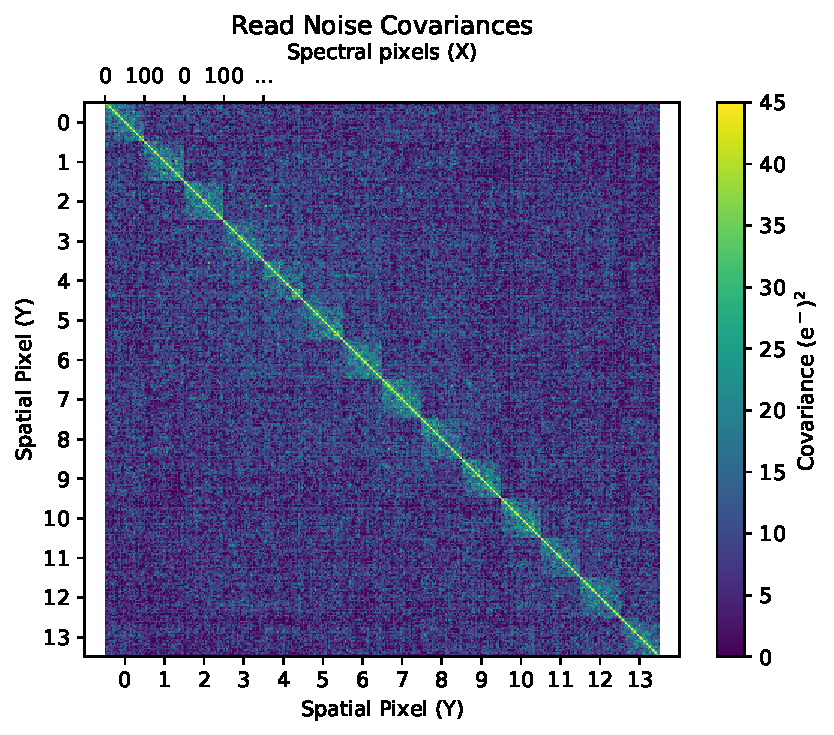
\includegraphics[width=.49\columnwidth]{spec_spatial_cov.pdf}
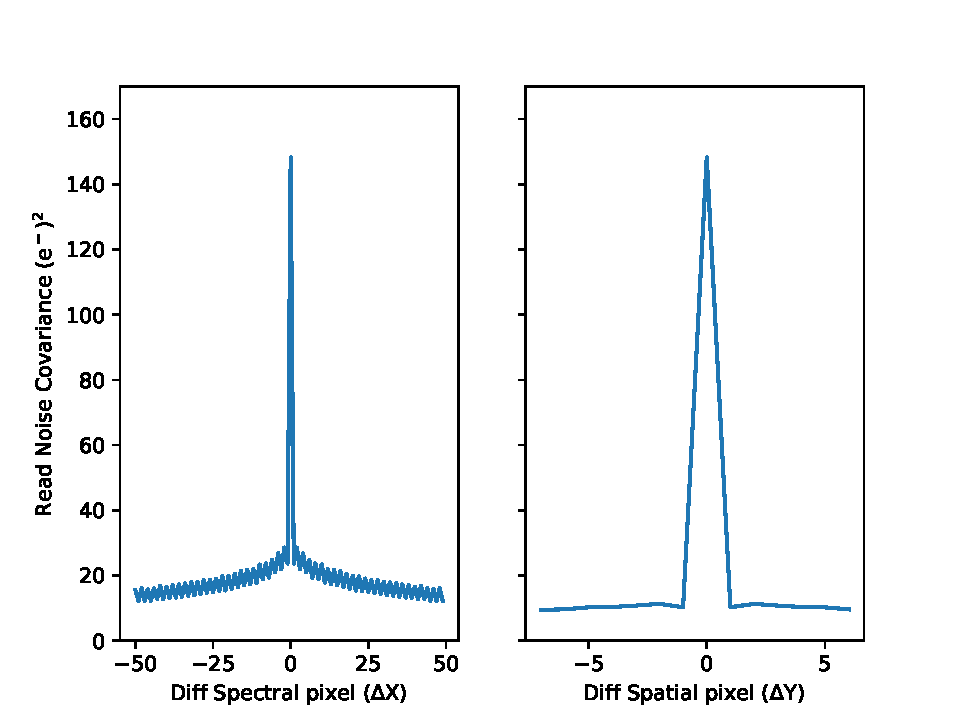
\includegraphics[width=.49\columnwidth]{cross_sections_cov.pdf}
\caption{{\it Left:} The read noise shows significant correlations between pixels -- unlike the traditional assumption that each pixel's noise is statistically independent.
The data was computed from a long dark exposure of 54 read pairs where reference pixel corrections, column-by-column subtraction and row-by-row subtraction have been performed.
The detector's diagonal elements are slightly below the published detector read noise ($13^2 = 169 (e^-)^2$) due to the row-by-row and column-by-column subtraction step.
{\it Right:} The spectral (X) and spatial (Y) directions from the matrix are averaged to build up a higher signal to noise covariance profile.
Spatially, the pixels have a covariance of 20~$(e^-)^2$ and a somewhat smaller spatial covariance of 10$(e^-)^2$.}\label{fig:covSpecSpatial}
\end{figure}

\subsubsection{Empirical Covariance Matrix}\label{sec:empCovarianceMatrix}
The ideal weighting of the spectrum from Equation \ref{eq:covarianceweights} depends on the covariance matrix $C_{ij}$.
We use a long dark exposure from the Optical Telescope Element and Integrated Science test performed at NASA Johnson on August 23, 2017 to estimate the read noise in $C_{ij}$.
We process the data by performing a CDS (correlated double sampling) read pairs of long dark data (108 frames) with reference pixel corrections, column-by-column median subtraction and row-by-row median subtraction.
These represent the steps that will be performed on grism time series before extraction.
We consider a wavelength bin that is 100 pixels in the dispersion direction (0.1$\mu$m) and 14 spatial spatial pixels.
The resulting images are similar to Figure \ref{fig:longDarkPhot} (right).

Figure \ref{fig:covSpecSpatial} shows the covariance matrix of this wavelength bin, taken from the median covariance matrix of 20 regions of the detector.
The diagonal elements $\sim 150 (e^-)^2$ are smaller than published NIRCam detector performance tables ($\sigma^2 \approx 13^2 (e^-)^2=169 (e^-)^2$).
However, if we skip the row-by-row and column-by-column subtraction step, they are consistent with $\sigma^2 \approx 13^2 (e^-)^2=169 (e^-)^2$.
It is clear that 1/f noise causes covariance most prominently along the spectral direction (the fast-read direction), with a covariance near 20~$(e^-)^2$.
Surprisingly, there is also a covariance between spatial pixels (the slow read direction) of $\sim$10 $(e^-)^2$.

The empirical covariance matrix from Figure \ref{fig:covSpecSpatial} is used to estimate the optimal pixel weights using Equation \ref{eq:covarianceweights}.
We reduce the noise and jaggedness of the empirical covariance matrix in Figure \ref{fig:covSpecSpatial} by averaging the value along the diagonal, across all spectral pixels and across the spatial pixels with the same value of $i -j$.
Here, the profile is the value from \texttt{pynrc}, which uses \texttt{webbpsf}.
We assume that the photon and background noise is $\sqrt{N_{phot}}$ and that they are completely uncorrelated from on pixel to next, so the covariance matrix is the sum, in quadrature, of the empirical read noise covariance matrix and a diagonal photon noise matrix.

The resulting optimal weighting function $w_j/P_j$ is plotted in Figure \ref{fig:covWeightedSummation}.
This optimal weighting significantly increases the contributions from the inner pixels compared to variance weights.
The optimal weighting scheme also negatively weights some pixels outside the core of the PSF to reduce correlated noise.

\begin{figure}[!hbtp]
\centering
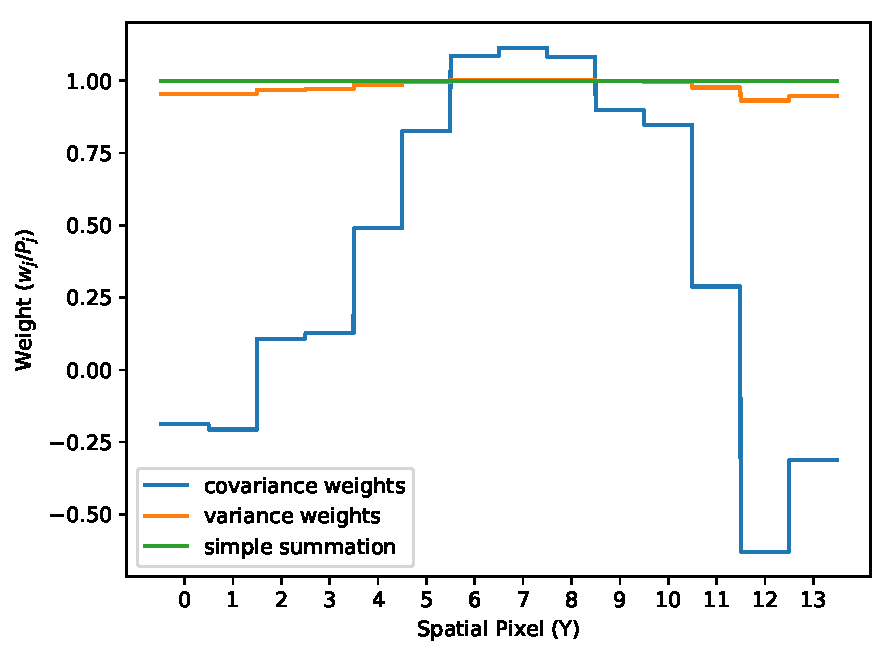
\includegraphics[width=.66\columnwidth]{cov_weighted_weights.pdf}
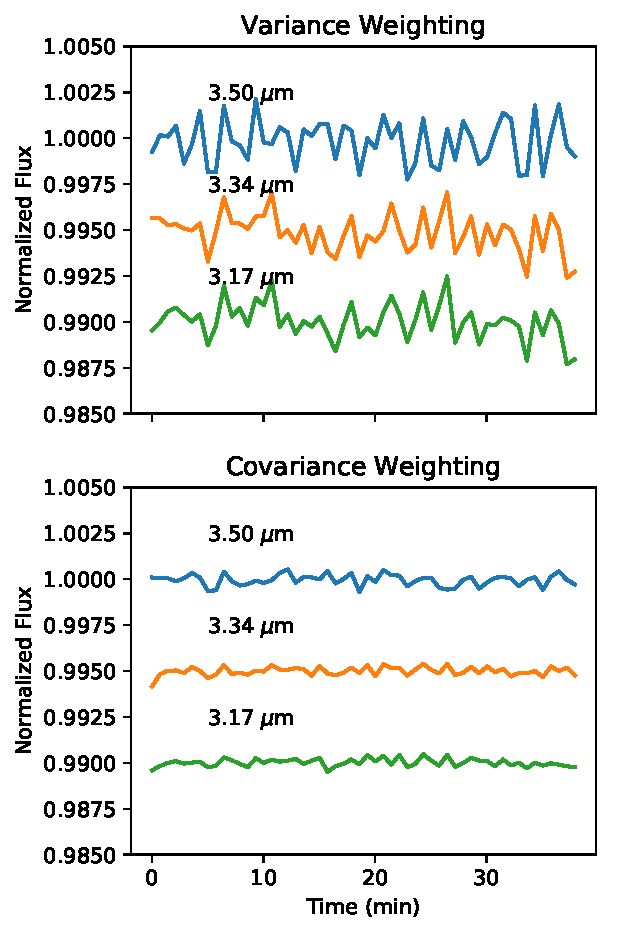
\includegraphics[width=.32\columnwidth]{zoom_cov_vs_var_tser.pdf}
\caption{ {\it Left:} Covariance weighting using the empirical covariance matrix has more severe weighting than simple summation and conventional variance weighting used in optimal extraction. {\it Right:} Covariance weighting will dramatically lower the scatter in the dark frame time series compared to variance weighting.}\label{fig:covWeightedSummation}
\end{figure}

Optimal covariance weighting significantly lowers the contribution of read noise to the overall error budget.
We test this with a series of grism images with a constant spectrum of an A0V star added to the CDS read pairs, but do not add photon noise to focus on the read noise contribution.
We do background subtraction along the dispersion and spatial directions, as would be done in a spectroscopic extraction pipeline.
We perform sum extraction over a 15 spatial pixels and then combine together 165 spectral pixels into a 0.165 $\mu$m wavelength bin.
The standard deviation of sum extraction is 3,860 DN, which is 2.7$\times$ the read noise, as shown in Table \ref{tab:noiseSummary1overf}.
The standard deviation of the extracted flux drops to 3,060 DN if optimal extraction is used.

We use Equation \ref{eq:covarianceweights}, to further reduce the read noise.
For the covariance weights, we assume constant off-diagonal weights of 15 (e$^-)^2$ and do not include the spectral covariance.
The resulting standard deviation of 850 DN is now 60\% of the photon noise.
Thus, we recommend optimal covariance weighting when extracting grism time series.
As the number of groups of the ramp is increased, the read noise should drop as 1/$\sqrt{N_G}$ so the covariance weighting most important when $N_G$ is small.

The methodology in calculating $P_j$ and Cov($S_i,S_j$) can significantly affect the precision on the time series.
Typically $P_j$ and the photon noise contribution to Cov($S_i,S_j$) can be found by fitting smooth functions (polynomials) along the dispersion direction.
If $P_j$ is calculated from each image individually, it will inherit the 1/f noise variations of each image.
Therefore, we hold $P_j$ constant along the time series with a value saved from the middle image at all wavelengths.
Alternatively, $P_j$ could be calculated from a PSF library or theoretically from \texttt{WebbPSF} \citep{perrin2014webbpsf}.

%% See the notebooks wlp8_psf_image.ipynb and noise_sources_wlp8.ipynb for calculations
\subsection{The impact of correlated read noise on time series}

\begin{figure}[!hbtp]
\centering
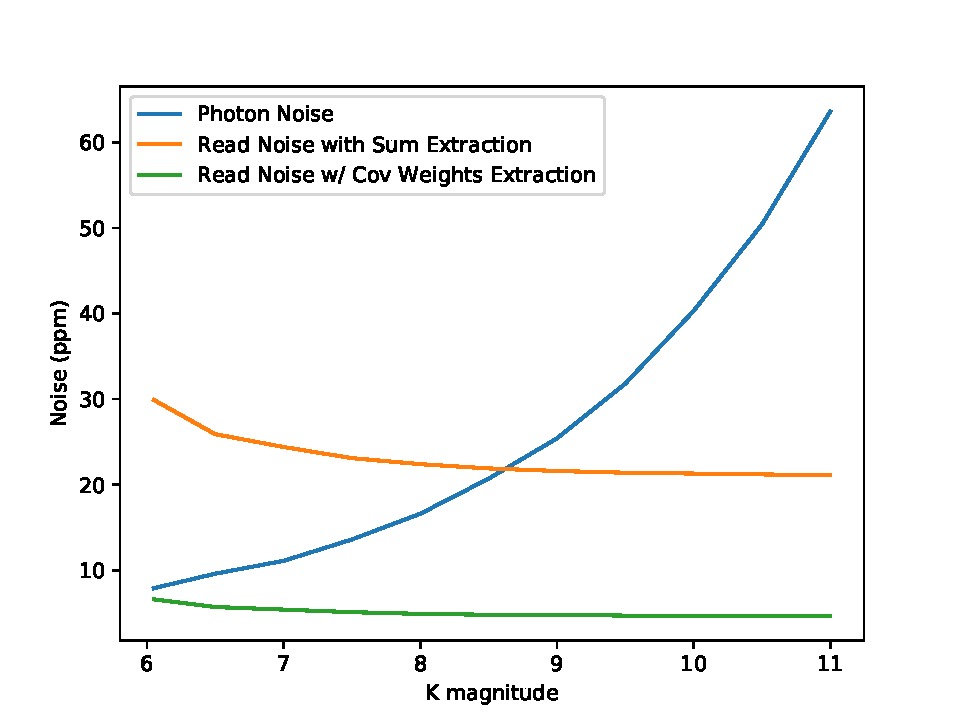
\includegraphics[width=.49\columnwidth]{generic_src_errors.pdf}
\caption{Bright sources, where only a handful of groups per integration are possible without saturation, can be dominated by read noise if simple sum extraction is used.
A covariance-weighted extraction can substantially decrease the contribution of correlated read noise to below the photon limit.
The errors here are for a grism time series wavelength bin that is 0.17$\mu$m wide centered on 3.34 $\mu$m for a G-type host star and a 3 hour transit duration.
}\label{fig:genericSourceErrorContrib}
\end{figure}

So far, we have discussed the magnitude of correlated read noise on an integration-by-integration basis, but here we explore how it will impact science.
We calculate the expected noise in the transit depth or eclipse depth of a generic exoplanet.
For this calculation, we assume a planet orbits a G-type 5800 K star, has a 3 hour transit duration and is observed with a 2048$\times$256 stripe subarray and is read out in RAPID mode with 1 frame per group and 4 amplifiers (No. of output channels=4).
We consider a range of $K$ magnitudes from 6 to 11.
We then calculate the maximum number of groups up the ramp that can be commanded while keeping the peak pixel count below 50\% well depth to safely avoid severe non-linearities.
From there, we calculate the noise due to photon counting statistics (ie. $\sqrt{N_{phot}}$) and compare it to the read noise.
As in Section \ref{sec:GrismDarkExtraction}, we focus on a 0.17~$\mu$m wide bin centered at 3.34~$\mu$m

Figure \ref{fig:genericSourceErrorContrib} shows the photon noise as a function of $K$ Vega magnitude.
The photon noise scales as $\sqrt{f}$, where $f$ is the flux because it is in the foreground limit.
The read noise drops slowly with $K$ magnitude because the time to reset between integrations takes a smaller and smaller fraction of the total exposure as the number of groups per integration grows.
We show the read noise assuming sum extraction (1044 ppm for CDS integration) and covariance-weighted extraction using Equation \ref{eq:covarianceweights} (230 ppm for CDS integration).
If a sum extraction is used, the read noise will dominate for $K \lesssim 8.7$.
However, covariance weights can ensure that photon shot noise is more dominant.

Some of the most interesting targets will be nearby bright sources, where the photon noise is small and the feature size is small.
For context, the features size of atmospheric signatures on archetypical planets are expected to be $\sim$300~ppm for hot Jupiters and Neptunes but only 10 ppm for cool Super-Earths like K2-3 b if they have high metallicity atmospheres \citep{greene2016jwst_trans}.
Therefore, observations of transiting cool super-Earths will require careful treatment of the correlated read noise, such as the covariance weighting scheme, to achieve the precision needed to probe their atmospheres.


We note that Figure \ref{fig:genericSourceErrorContrib} shows a somewhat counter-intuitive result: read noise dominates for bright source and becomes less important for faint sources.
For typical observations, such as faint galaxies or distant stars, the opposite is true: read noise is more of a concern for faint sources than bright ones.
So why is there a discrepancy?
The difference in these two science cases is that for exoplanet transit observations, the detector well depth is filled to approximately the same level ($\sim 32,000$ DN or 50\% well depth per pixel) regardless if the system's magnitude is 6 or 11.
For the bright source with a few groups up the ramp, the read noise will be a larger fraction of 32,000 DN than for a faint source with many groups up the ramp.
This is different from a faint galaxy in the $K > 20$ range, which will not fill the detector well.
For a fixed exposure time, a $K=25$ and $K=20$ galaxies would be observed with approximately the same number of groups per integration so the read noise in DN from each source in an integration would be approximately the same whereas the number of DN from the source per integration would be 100 times larger for the $K=20$ galaxy.

\section{Fringing}

The thin layer of NIRCam's HgCdTe detector can result in an interference pattern much like thin film interference on bubbles.
Fringing will be less noticeable when many wavelengths are mixed together, but with grism spectra where the wavelengths are separated, the interference effects are more pronounced.
We investigate whether this can manifest itself on the spectrum with the NIRCam grism by looking for periodic signatures that vary in frequency as a function of wavelength.

\begin{figure*}[!hbtp]
\centering
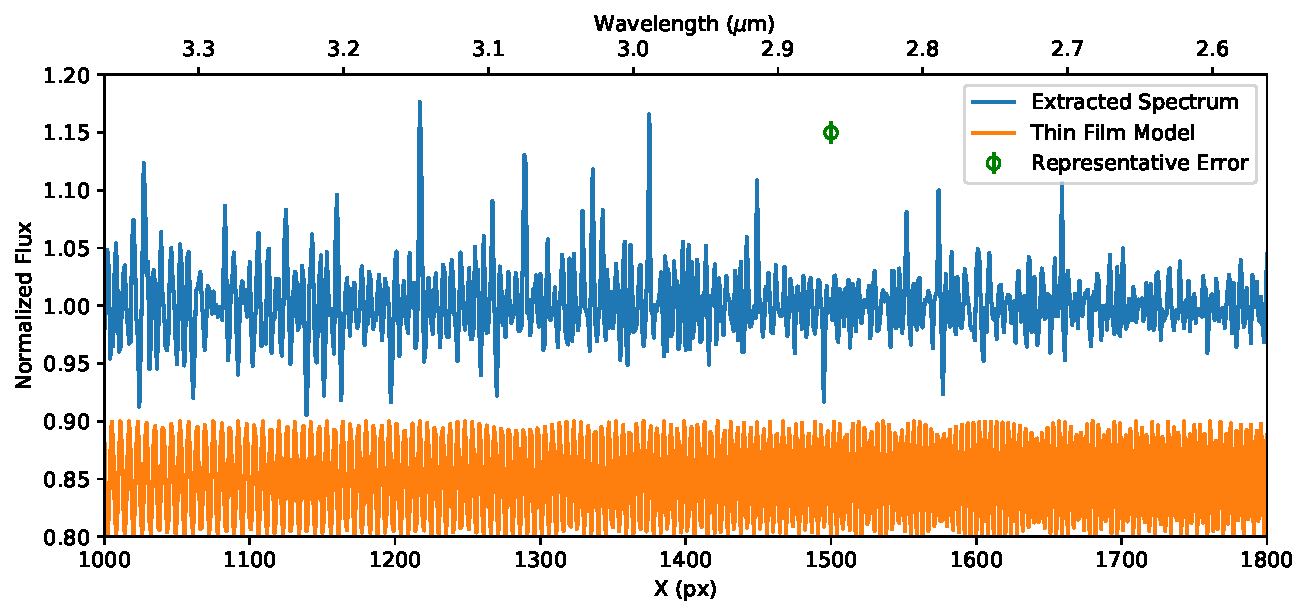
\includegraphics[width=.99\columnwidth]{fringing_grism_cv3.pdf}
\caption{A CV3 grism spectrum over the time series grism test shows evidence for fringing and where the oscillations exceed the photon and read noise (green point).
An illustrative sinusoidal function is plotted for comparison to better see how the frequencies change as a function of wavelength (X pixel).
}\label{fig:CV3GrismSpecFringing}
\end{figure*}

Figure \ref{fig:cv3ExtractedSpectrum} shows an extracted spectrum from Cryogenic Vacuum 3 testing at NASA Goddard where a broadband point source is dispersed by the grism.
The slope image is calculated from the raw ramp using the internal NIRCam ramps-to-slopes pipeline \texttt{ncdhas}.
The background is subtracted with a 2nd order polynomial fit and the flux is extracted with a variance-weighted summation \citep[e.g.][]{horne1986optimalE}.
The spectrum is normalized by a 3rd order spline fit with 400 knots to remove the broad shape of the spectrum and the throughput curves.
The resulting spectrum shows high frequency ($\sim$0.2 px$^{-1}$ to $\sim$0.5 px$^{-1}$) variations far in excess of the photon and read noise.
These oscillations increase in frequency at longer wavelengths (X pixels).
The variations have peak-to-valley amplitudes of about 8\%.
Figure \ref{fig:cv3ExtractedSpectrum} also shows an illustrative fringing model that increases in frequency as the wavelength decreases.

The fringing pattern is clearly visible in the grism spectrum, so it will be imprinted on all grism spectra.
However, this fringing pattern should be a function of the detector thickness and should remain constant for a fixed position in the detector.
The grism time series observations will be performed with target acquisition to reliably centroid on the source to better than 0.15 long wavelength pixels.
We therefore expect that the fringing pattern will be repeatable from one observation to the next.
For use in stellar characterization, however, it may be helpful to divide this fringing pattern out from a correction function made from a standard star.


\section{Subpixel Crosshatching}

\subsubsection{Subpixel Crosshatching Characterization}
The flat field of the ALONG detector, which is used for NIRCam grism series, has a pronounced crosshatch pattern visible in Figure \ref{fig:crossHatchA5}.
The patterns are located at 23.1$\degree$ , 90.9$\degree$, and 158.6 $\degree$ counter-clockwise from the $+$X direction of the detector.
The angle between these lines are 67.8$\degree$, 67.7$\degree$ and 44.5$\degree$.
These angles and patterns can be analyzed with a 2D power spectrum as shown in Figure \ref{fig:crossHatchA5}.


\begin{figure}[!hbtp]
\centering
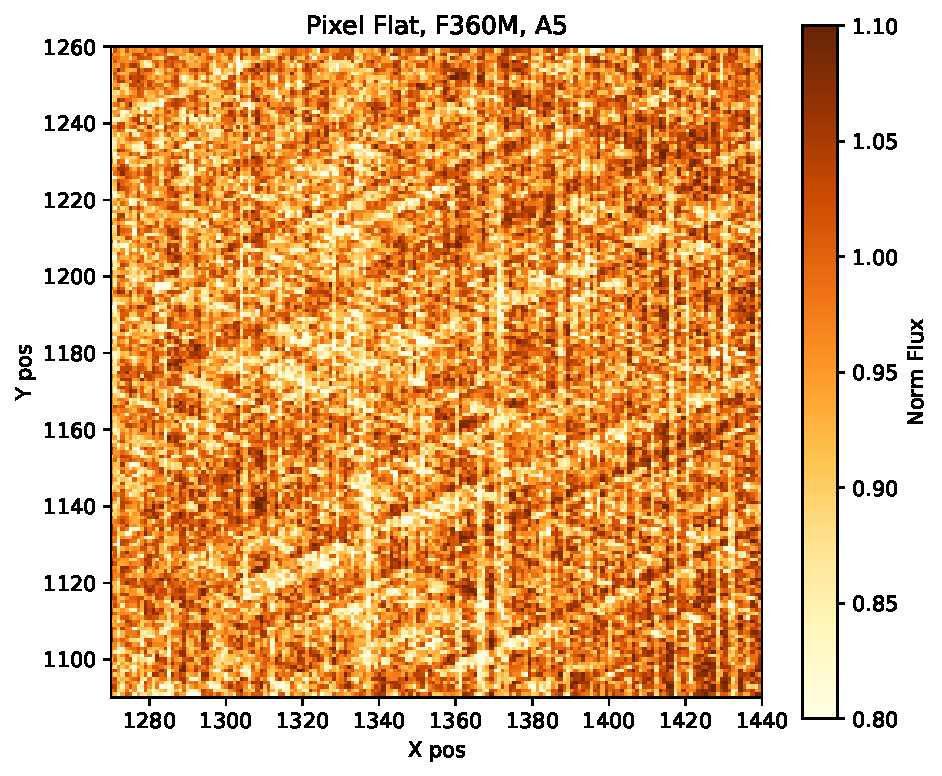
\includegraphics[width=.49\columnwidth]{crosshatch_zoom.pdf}
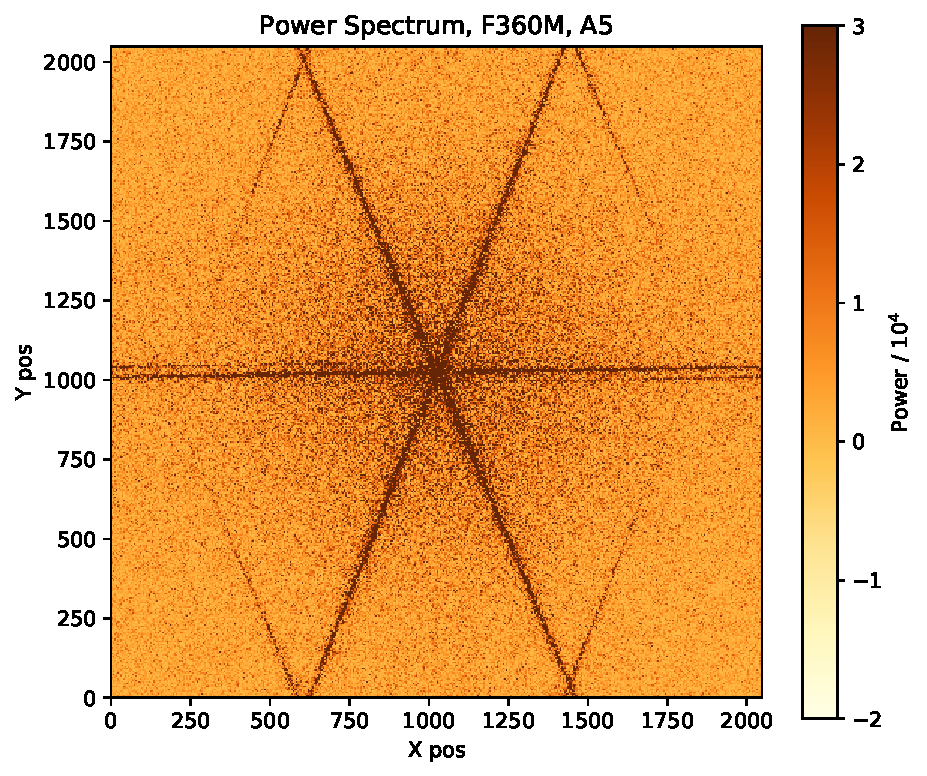
\includegraphics[width=.49\columnwidth]{crosshatch_2d_power.pdf}
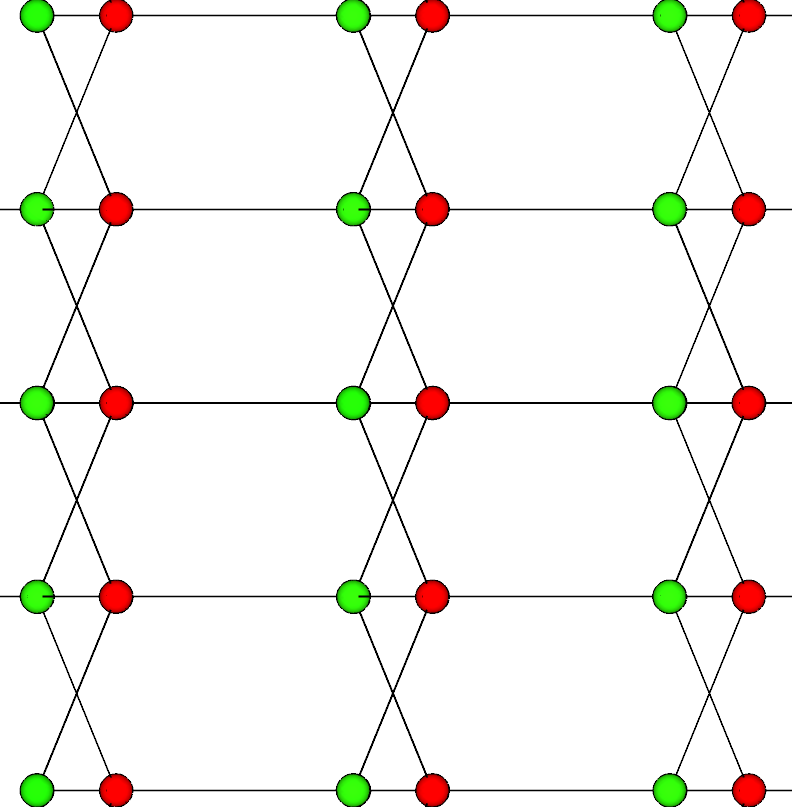
\includegraphics[width=.3\columnwidth]{tetrahedral_lattice_projection.png}
\caption{
The A5 detector's flat field has a pronounced crosshatch pattern at 23.1$\degree$ , 90.9$\degree$, and 158.6 $\degree$ CCW from the positive X direction.
The crosshatch pattern is visible in a zoom-in of the pixel flat field (top left).
The 2D power spectrum of the flat field (top right) shows a continuum of frequencies aligned with the three crosshatch angles.
Note the lines in frequency plane are perpendicular to the crosshatch directions in the image plane.
These three relative crosshatch angles (67.8$\degree$, 67.7$\degree$ and 44.5$\degree$) are similar to a projection of a tetrahedral (zincblende) lattice structure of HgCdTe (bottom, 67.8$\degree$, 67.8$\degree$, 44.4$\degree$).
}\label{fig:crossHatchA5}
\end{figure}

The angles of the crosshatch patterns are determined by the crystal pattern of HgCdTe.
HgCdTe has a zincblende structure with tetrahedral bond angles where each Hg or Cd atom is surrounded by 4 Te atoms \citep{gemain2012mercVacanciesHgCdTe}.
HgCdTe detectors are manufactured using molecular beam epitaxy upon a substrate, a process which can result in topological defects with peak to valley amplitudes of 5-20 nm in height variations \citep{chang2008surfaceMorphologyHgCdTe}.
The surface morphology of the HgCdTe crystal shows that the crosshatch patterns are are oriented along the intersection of the (211) growth plane of the crystal and the 8 HgCdTe slip planes.

The relative angles of the HgCdTe slip planes and (211) growth plane are 44.42$\degree$, 67.79$\degree$ and 67.79$\degree$ \citep{chang2008surfaceMorphologyHgCdTe}, very close to the observed crosshatch angles.
A projection of zincblende structure is shown in Figure \ref{fig:crossHatchA5} relative to the observed crosshatch patterns.
The similarity between the crosshatch patterns in the flat field and the topological variations observed in \citet{chang2008surfaceMorphologyHgCdTe} leads to the likely conclusion that the surface variations lead to quantum efficiency variations.
Thus, the crosshatch pattern is mostly likely related to the crystal lattice structure of the HgCdTe substrate and not the pixel circuitry.

The crosshatch structure of the detectors extends down to the subpixel level, so it will not be fully corrected with a flat field division.
This sub-pixel structure has been imaged with microscopy on a Euclid HgCdTe detector \citep{shapiro2018crosshatch}.
Atomic force microscopy shows topological features that are approximately 1.2~$\mu$m in width \citep{chang2008surfaceMorphologyHgCdTe} compared to the 18~$\mu$m pixel sizes.
The width of the structures can also be estimated from the behavior for crosshatch lines as they cross pixel boundaries \citep{ninan2019crosshatchHPF}.
We estimate that the crosshatch pattern oriented at 90.9$\degree$ crosses 1 horizontal pixel for every 64 vertical pixels.
While crossing the boundary, there are $\approx 38$ rows where the crosshatch pattern spans more than 2 pixels.
If the crosshatch pattern has a tophat response function, then these 38 rows where the pattern spans two pixels imply a tophat full width of 0.6 pixels or a physical width of 10.8~$\mu$m for an 18~$\mu$m pixel pitch.
This is more than twice the estimate from \citet{ninan2019crosshatchHPF} for an HgCdTe used on the Habitable Planet Finder.
We expect that the crosshatch pattern's width varies among detectors or that a tophat function is a poor approximation of the actual subpixel response.
Within NIRCam detectors, there are large variations in the strength and orientation of crosshatch features.

The crosshatch pattern is wavelength dependent, as seen in Figure \ref{fig:crossHatchWavelengthDep}, where the throughput variations are the largest for short wavelengths (better resolving crystal structures) and smallest for the long wavelengths.
This is visible both in the throughput cross section of the flat field and the Fourier amplitude of the crosshatch as a function of wavelength.
We find a steeper wavelength dependence to the crosshatch pattern near 0.9$\degree$ from horizontal in the frequency domain or 0.9$\degree$ from vertical in the length domain.
%We also fit the crosshatch pattern.

\begin{figure}[!hbtp]
\centering
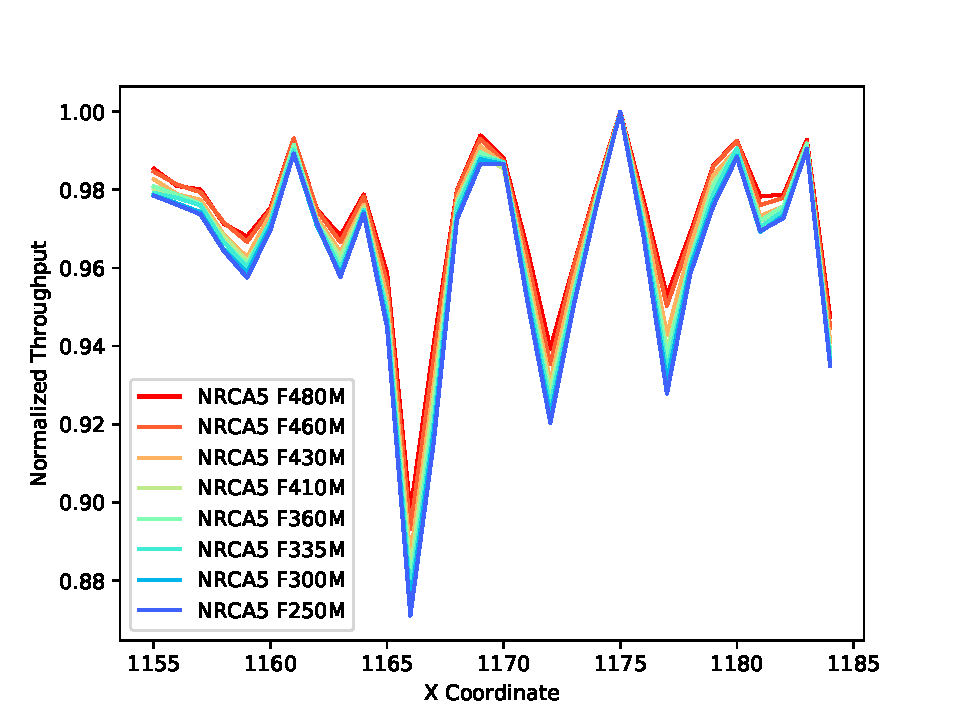
\includegraphics[width=.49\columnwidth]{cross_sec_of_crosshatch.pdf}
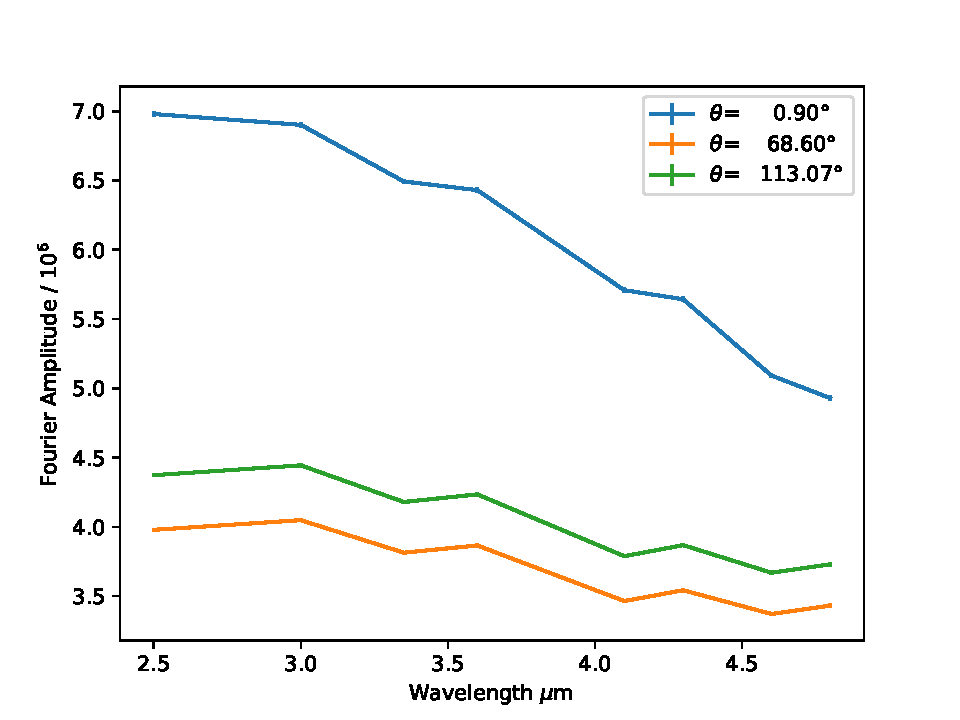
\includegraphics[width=.49\columnwidth]{fourier_power_from_fit.pdf}
\caption{
The crosshatch pattern changes as a function of wavelength, possibly because the shorter wavelengths resolve the structure better.
The shorter wavelengths have deeper crosshatch troughs (left) and higher Fourier amplitudes (right).
}\label{fig:crossHatchWavelengthDep}
\end{figure}


\subsection{Crosshatch Pattern Modeling}\label{sec:crosshatchModeling}
We model the crosshatch pattern in the Fourier space because it has a smoother pattern as a function of spatial frequency than in spatial coordinates as seen in Figure \ref{fig:crossHatchA5}.
We divide the 2D Fourier power spectral density by the number of pixels in an input image.
This was experimentally determined to give a power spectral density that does not change with the dimensions of the input image.
\textcolor{red}{Can we justify this more? I thought it would be pixels$^2$}

We model the two dimensional Fourier power spectral density $f(k_{x,i}',k_{y,i}')$ for one angle $\theta_i$ as
\begin{equation}\label{eq:analyticPSDradial}
f(k_{x,i}',k_{y,i}', a_i, b,c) = a_i \exp{\left(- |k_{x,i}'| / b \right)} \left( \frac{1}{(0.5 c)^2 + k_y'^2} \right),
\end{equation}
where $k_x'$ and $k_y'$ are rotated frequency coordinates in the parallel and perpendicular directions, $a$ is the amplitude, $b$ is the parallel exponential constant and $c$ is the Lorentzian full width at half maximum of the perpendicular dependence.
For each of the three angles, there is a set of rotated coordinates centered at $(k_{x,0},k_{y,0})$= (0,0) following:
\begin{equation}
k_x'(\theta_i) = k_x \cos{\theta_i} + k_y \sin{\theta_i}
\end{equation}
and
\begin{equation}
k_y'(\theta_i) = -k_x  \sin{\theta_i} + k_y \cos{\theta_i}.
\end{equation}
We include three angles so that the total power spectral density is
\begin{equation}\label{eq:fullPSDmodel}
f(k_x,k_y) = \sum_{i=1}^{i=3} f_i(k_{x,i}'(\theta_i),k_{y,i}'(\theta_i),a_i,b,c) + d \exp{\left(-k_r/e_b\right)},
\end{equation}

This model has 8 free parameters: three angles ($\theta_i$, three amplitudes ($a_i$), a joint parallel exponential constant ($b$) and joint Lorentzian width ($c$).
Finally, we include an exponential term that fits the broad azimuthally symmetric background to all the power spectra,
where $d$ is the amplitude of the radial ``background'', $k_r= \sqrt{k_x^2+k_y^2}$ is the radial frequency and $e_b$ is the radial background exponential constant.
We only fit the region of the power spectral density above frequencies of 0.05 px$^{-1}$ to focus on the high frequency component of the flat field where the crosshatch is most prevalent.

For the F300M filter and ALONG detector, we find 
for $\theta_1 = 0.906 \pm 0.001 \degree, \theta_2 = 68.605 \pm 0.001 \degree, \theta_3 = 113.075 \pm 0.001, a_1 = 2.774 \pm 0.002 \times 10^{-7}, a_2 = 1.569 \pm 0.002 \times 10^{-7}, a_3 = 1.744 \pm 0.002 \times 10^{-7}, b=0.345 \pm 0.0005 $ px$^{-1}$, $c=2.05 \pm 0.07 \times 10^{-2}$ px$^{-1}$, $d=6.78 \pm 0.01 10^{-3}$ and $e_b=0.26 \pm 0.01$ px$^{-1}$.
In other words, the separations between the vectors are $67.699 \degree, 67.831 \degree$, and $44.470 \degree$.
The uncertainties were simply derived from the diagonals of the covariance matrix and may be underestimated.

\begin{figure}[!hbtp]
\centering
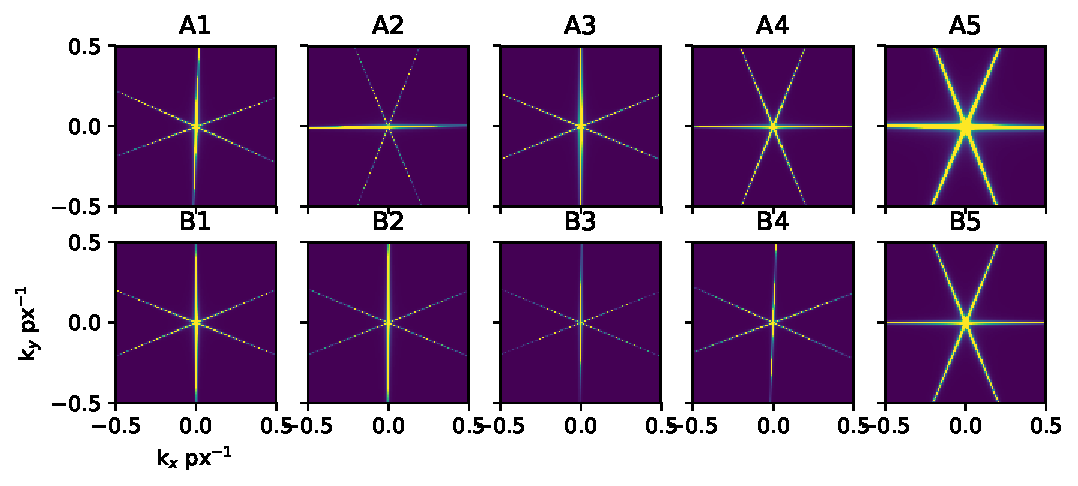
\includegraphics[width=.99\columnwidth]{psd_models_gallery.pdf}
\caption{
Best-fit power spectra of all the NIRCam detectors show that the long wavelength detectors A5 and B5 show the most pronounced crosshatch patterns.
The primary crosshatch tends to be aligned closely, but not exactly, with either the X or Y axis.
The images have all been normalized to the same scale to show the relative crosshatch amplitudes of different detectors.
}\label{fig:crosshatchModelGallery}
\end{figure}

NIRCam's 10 SCA's have very similar crosshatch angles with separations of 44.5 $\degree$ and 67.7 to 67.8 $\degree$ as seen in Figure \ref{fig:crosshatchModelGallery}.
They all have one primary crosshatch axis oriented either along the X pixels or the Y pixels, with two flanking axes at $\sim 67.7 \degree$ to either side.
The long wavelength arrays have a more pronounced crosshatch than the short wavelength arrays.
The NRCB4 array's primary crosshatch direction is most closely aligned with a pixel axis (the Y direction) than any SCA.
Figure \ref{fig:crosshatchModelGallery} shows the best-fit crosshatch 2D power spectra.


\subsection{Position of SubGrism Array}

The crosshatch pattern varies in amplitude and angular dependence from one physical location on the detector to another.
The ALONG detector has more pronounced crosshatching toward the middle of the detector that falls off toward the perimeter.
On the other hand, the BLONG detector has more pronounced crosshatching towards the boundary.
We fit the crosshatch pattern to three regions of the ALONG detector, which is the one used for the NIRCam grism time series mode:
\begin{enumerate}
	\item The 2048$\times$64 SUBGRISM position at the bottom of the array where the bottom left corner is (4,5) \label{subgrism64pos}
	\item A 2048$\times$64 theoretical subarray at the top of the ALONG detector where the bottom left corner is (4,1984)
	\item A 2048$\times$64 cutout of the full frame detector that is centered on the grism time series field point.
\end{enumerate}

\begin{figure}[!hbtp]
\centering
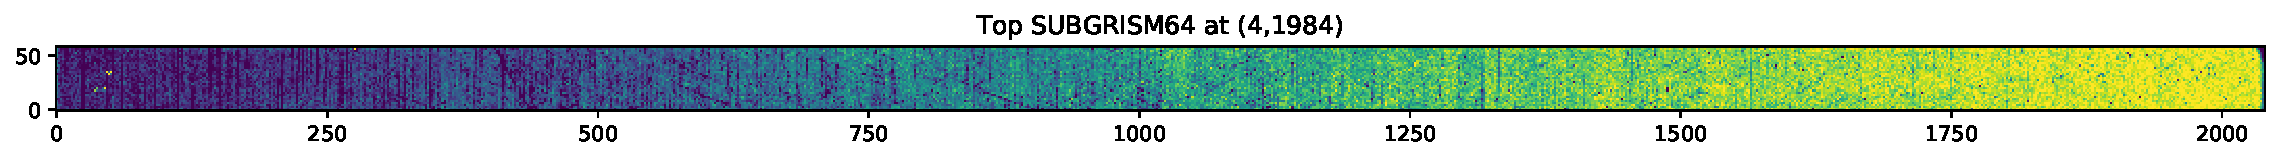
\includegraphics[width=0.99\columnwidth]{subg_pos_topGrism64.pdf}\\
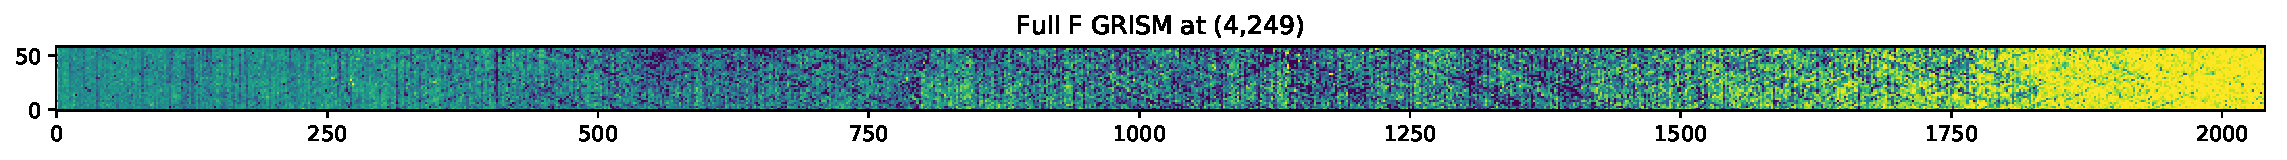
\includegraphics[width=0.99\columnwidth]{subg_pos_fullfGrismRegion.pdf}\\
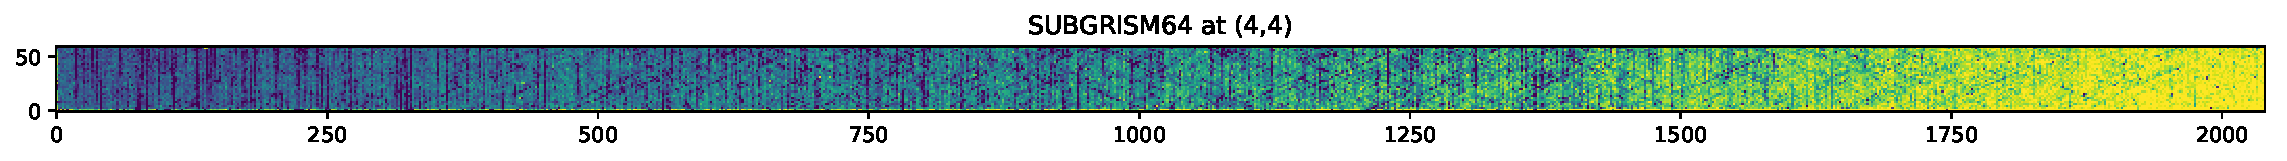
\includegraphics[width=0.99\columnwidth]{subg_pos_subgrism64.pdf}\\
\vspace{0.2in}
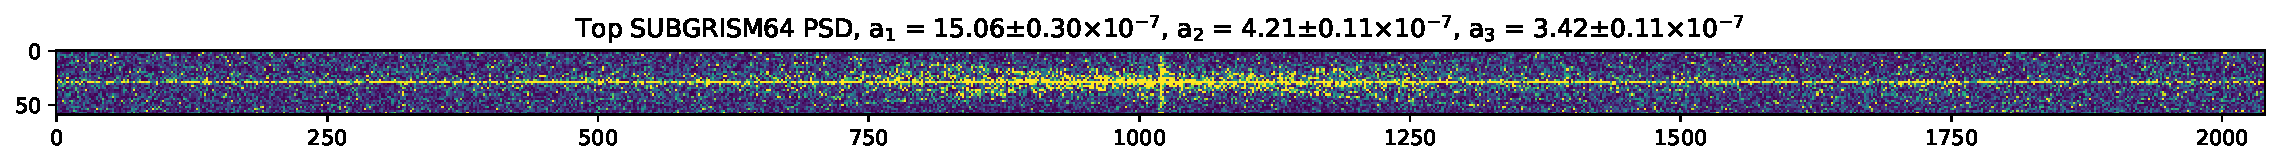
\includegraphics[width=0.99\columnwidth]{subg_pos_topGrism64_psd.pdf}\\
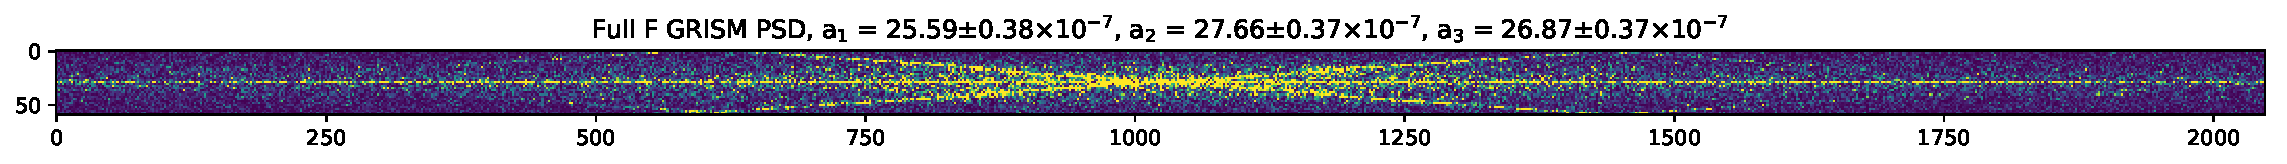
\includegraphics[width=0.99\columnwidth]{subg_pos_fullfGrismRegion_psd.pdf}\\
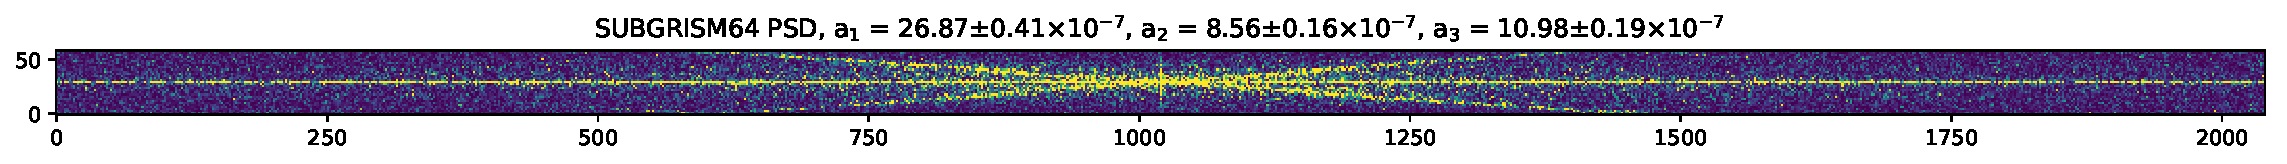
\includegraphics[width=0.99\columnwidth]{subg_pos_subgrism64_psd.pdf}\\
\caption{
The top of the array has the smallest level of crosshatching and the middle has the largest.
This is visible in the flat field images (top three panels) and their power spectral density functions (bottom three panels) for three different sections of the A5 detector: a theoretical ``aperture'' position at the top of the array (first plot from top), the full frame position near Y=512 (second plot from top) and the nominal SUBGRISM64 at the bottom of the array (third plot from top).
The bottom left corner for each subarray is listed in parentheses in the title of the flat field plot and the best-fit amplitudes are listed in the title of the power spectral density plot.
 }\label{fig:crosshatchGrismPos}
\end{figure}

The three subarrays considered are shown in Figure \ref{fig:crosshatchGrismPos}.
We exclude reference pixels (which form a 4 pixel wide boundary around the detector) and an additional row on the bottom and top of the array because these illuminated rows are outliers in the flat field.
The first position is nearly the same as the SUBGRISM64 subarray position in the grism time series mode, except that the SUBGRISM64 includes the first 5 rows which are excluded here from the crosshatch analysis.
The field point used for the SUBGRISM64 mode is expected to be the same one as will be used for the SUBGRISM128 and SUBGRISM256 subarrays.
The position at the top of the ALONG detector has the smallest amplitude of crosshatch pattern in all three directions.
The best-fit amplitudes are used as input to the jitter simulations in Section \ref{sec:CrosshatchSim}.
We find that the maximum flux change for a 0.1 pixel shift is 118 ppm for the nominal grism position, 108 ppm for the top of the array and 153 ppm at the full frame grism position.

\subsection{Subpixel Crosshatching Calculation}\label{sec:CrosshatchSim}

The subpixel crosshatch pattern can potentially introduce time-variable noise as the point spread function drifts with telescope pointing drifts, long timescale jitter.
NIRCam observations are expected to have a root-mean-square deviation of 6.0 mas in each axis when measured in 15 second intervals over a 10,000 second observation.\footnote{See \url{https://jwst-docs.stsci.edu/display/JTI/JWST+Pointing+Performance\#JWSTPointingPerformance-Pointing\_stabilityPointingstability}}

We simulate the effect of this jitter on NIRCam time series observations with the following steps:
\begin{enumerate}
	\item Fit the existing flat field to a crosshatch model in the Fourier domain
	\item Extrapolate the crosshatch model to higher frequencies (30 px$^{-1}$) to estimate the sub-pixel structure
	\item Simulate an over-sampled PSF using \texttt{webbpsf} \citep{perrin2014webbpsf}
	\item Shift the PSF along the X and Y directions (as much as 6 mas) \label{it:xHatchShiftPSF}
	\item Multiply the PSF by the simulated flat field
	\item Bin the simulated images into the native pixel size
	\item Divide by the pixel-to-pixel flat field (as would be done in pipeline)
	\item Measure the relative flux with a photometric aperture with the same shift applied \label{it:xHatchApPhot}
\end{enumerate}

As discussed, in Section \ref{sec:crosshatchModeling}, we fit equation \ref{eq:fullPSDmodel} to the measured power spectral density of the F300M filter for the frequencies above 0.05 px$^{-1}$.
We evaluate equation \ref{eq:analyticPSDradial} for frequencies in the oversampled image from 0 px$^{-1}$ to 30 px$^{-1}$ and multiply this by the number of pixels and the square of the oversampling factor (ie. $60^2$) to convert from the scale-invariant Power Spectral Density to the simulated PSD.
We then assign random phases uniformly from 0 to 2$\pi$ for the complex Fourier plane because the original image's complex phase distribution is similar to uniform.
Finally, we take the real part of the inverse Fourier transform to create an oversampled image, as shown in \ref{fig:crossHatchSimPSF}.
For comparison to the original flat in Figure \ref{fig:crossHatchA5}, we binned to the oversampled flat field to the native LW pixel (1.0 native pixels=60.0 oversampled pixels $\approx$0.063 \arcsec).
This simulated pixel flat field with dimensions of 26 by 26 LW pixels has a peak of 1.15 to trough of 0.90 with a robust standard deviation of 0.05.
For comparison, the middle of the original F300M flat for the ALONG detector has a robust standard deviation 0.06.

\begin{figure}[!hbtp]
\centering
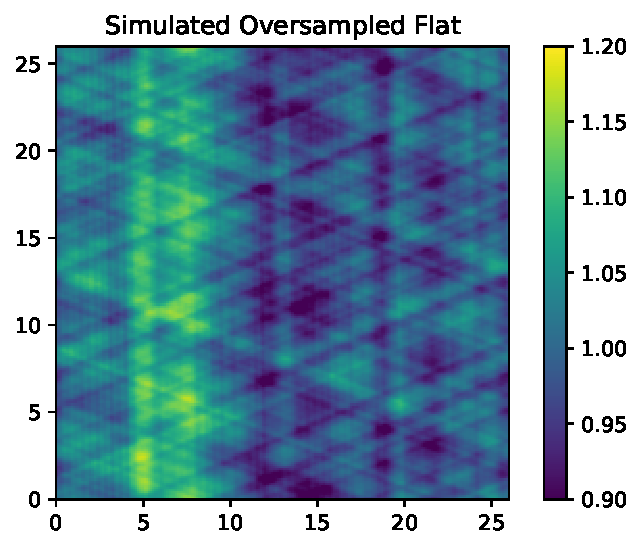
\includegraphics[width=.32\columnwidth]{sim_flat_Oversampled_plot.pdf}
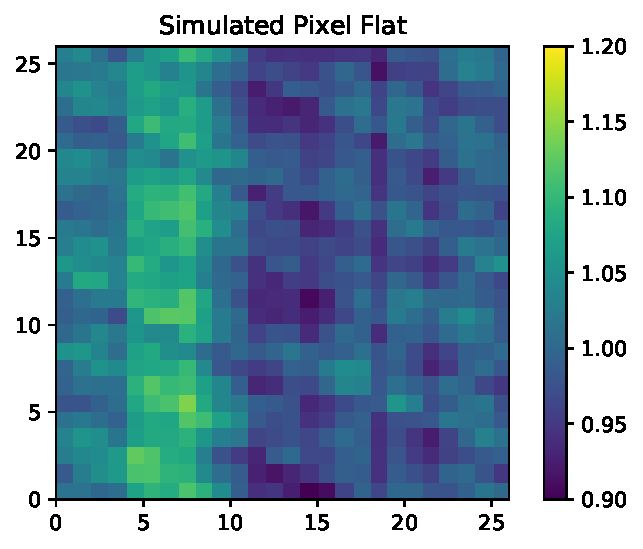
\includegraphics[width=.32\columnwidth]{sim_flat_Pixel_plot.pdf}
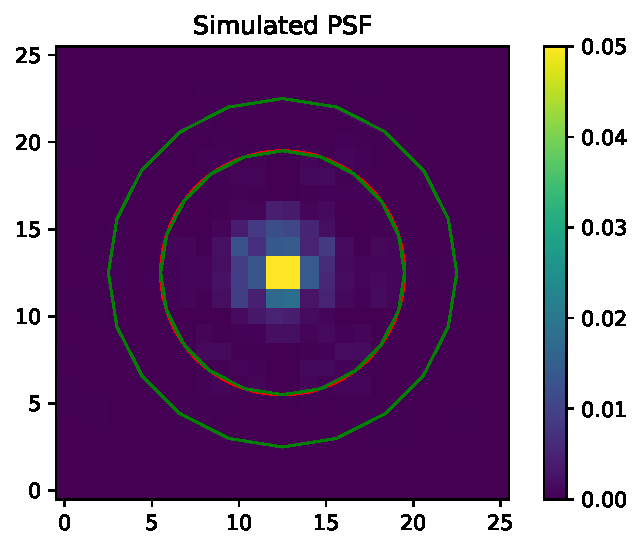
\includegraphics[width=.32\columnwidth]{psf_with_phot_ap_with_crosshatch.pdf}
\caption{
The steps of the sub-pixel crosshatch photometry simulation are shown here.
We simulate an over-sampled flat (left) by extrapolating the power spectrum to frequencies above the pixel sampling level.
This simulated flat is binned to the native pixel resolution to produce a pixel flat field (middle) that would be used by a standard pipeline that has no sub-pixel corrections.
A \texttt{WebbPSF} point spread function is created at the oversampled resolution, multiplied by the oversampled flat field and then binned to native resolution (right).
Finally, the simulated image is divided by the pixel flat field as would be performed in a standard pipeline reduction.
The simulated PSF shows the source and background apertures used in the simulation, which are centered on the PSF.
}\label{fig:crossHatchSimPSF}
\end{figure}

We next calculate a point spread function using \texttt{webbpsf} \citep{perrin2014webbpsf}, oversampled by a factor of 60.
\texttt{webbpsf} includes an optional blurring due to high frequency pointing jitter.
We set this Gaussian blurring parameter to 1 mas to simulate a worst-case scenario where the pointing drift is dominated by long-timescale behavior with minimal high frequency jitter.
We multiply the oversampled \texttt{webbpsf} source by the simulated oversampled flat and bin this to native pixel resolution to create a simulated observation as shown in Figure \ref{fig:crossHatchSimPSF}.
This simulated observation is divided by the binned simulated flat as would be done by a standard pipeline's flat field correction.

We repeat steps \ref{it:xHatchShiftPSF} through \ref{it:xHatchApPhot} of the observation simulation by shifting the over-sampled PSF by sub-pixel amounts.
The subpixel shifts of the over-sampled PSF are performed with \texttt{scipy.ndimage.shift}.
For each shifted PSF, we multiply this by the subpixel crosshatch pattern and bin the result.
These simulated operations represent pointing drift on the subpixel scale.

We calculate aperture photometry with a circular aperture with a radius of 7 pixels and a background annulus from 7 to 10 pixels on each of the observations.
The aperture is re-centered by the same position as the shift direction.
For each sub-pixel pointing drift, the aperture sum is subtracted by the background flux average per pixel multiplied by the pixel area of the source aperture.
While the simulations here include no background flux, we use the background subtraction to simulate the operations applied by a photometry pipeline.
These are also expected to be similar to a spectroscopic pipeline for a narrow spectral region or spectral line.
The differential flux between the centered PSF and the shifted one is shown in Figure \ref{fig:subpixScanSimulation}.


\begin{figure}[!hbtp]
\centering
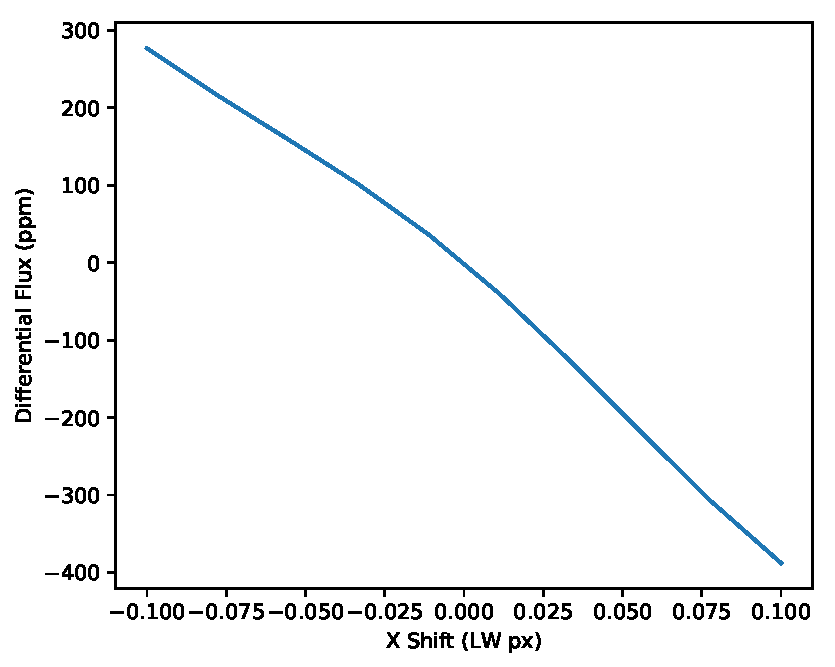
\includegraphics[width=.49\columnwidth]{scan_F300M_x_short_scan.pdf}
\includegraphics[width=.49\columnwidth]{scan_F300M_y_short_scan.pdf}
\caption{
The simulated subpixel crosshatch pattern from Figure \ref{fig:crossHatchSimPSF} for the F300M filter will cause spurious flux changes with small pointing drifts.
Here we show scans in the X direction and Y direction from the center of the image and a subpixel scale.
The amplitude of these scans is 6.3 mas for the $\sim$63 mas/px plate scale of the LW detector.
These are correctable with smooth functions such as polynomials.
}\label{fig:subpixScanSimulation}
\end{figure}

The subpixel crosshatch structure does indeed create flux variations with image motion as shown in Figure \ref{fig:subpixScanSimulation}.
The amplitude of the flux changes is potentially up to 150 ppm.
This is significant when compared to atmospheric features of giant planets ($\lesssim$ 100 ppm) or the transit depth of an Earth-like planet transiting a sun-like star ($\lesssim$ 80 ppm).

Fortunately, the subpixel crosshatch systematic is a smooth function of pointing drift, shown in Figure \ref{fig:subpixScanSimulation}.
A polynomial function can be fit to this subpixel dependence and then the centroid of each integration can be inserted as an argument to the function to provide a correction as a function of time.
Alternatively, a Gaussian process regression could be applied.
Centroiding is possible in imaging and spectroscopic modes using PSF fitting or cross-correlation.
When the LW grism time series mode is enabled, SW imaging data will automatically be collected simultaneously enabling the SW centroids to be used to track the motion of the dispersed grism image.
Furthermore, the pixels for time series modes can be characterized in detail because they will be re-used for all time series observations in a given mode.
Target acquisition is expected to achieve centroiding accuracy $\lesssim$ 10 mas ($\lesssim 0.15$ long wavelength pixels) for unsaturated target acquisition.\footnote{https://jwst-docs.stsci.edu/near-infrared-camera/nircam-operations/nircam-target-acquisition/nircam-time-series-imaging-target-acquisition}
This ensures that time series observations will reliably return to the same location within the same set of pixels with every visit.

\subsection{Time Series Simulation}
The JWST fine steering mirror (FSM) is designed to correct any telescope pointing errors that are not full corrected by the reaction wheels.
The JWST attitude control system team provided a simulation of the expected pointing performance shown in Figure \ref{fig:tserPointingFull}.

The dominant variations in the pointing in the simulation from Figure \ref{fig:tserPointingFull} are High Gain Antenna (HGA) moves.
These are moves are designed to keep the antenna pointing at ground-based antennas for telemetry or data download.
Fortunately, the errors due to HGA moves damp quickly on $\lesssim$ 1 minute e-folding timescales, as show in Figure \ref{fig:tserPointingZoom}.
This means that for 1 minute integrations, only about 1\% of integrations will be affected by HGA moves and the data for these moves could be discarded.
Other pointing errors can be caused by reaction wheel jitter, the MIRI cryocooler and fuel slosh in the fuel tanks.
The effect of the reaction wheels and MIRI cryocooler will be to blur the PSF over an integration since they are higher frequency $\gtrsim 1$ Hz.
Fuel slosh happens at the beginning of a visit after the telescope is slewed, but will dampen quickly on 100 second timescales.
Therefore, the largest contributor to pointing variations will likely be HGA moves and thermal inter-boresight motion.

\textcolor{red}{Once, we have thermal inter-boresight motion, show how this affects pointing/flux}

\begin{figure*}
\gridline{\fig{histos_v2_v3.pdf}{0.45\textwidth}{Pointing Histograms} 
\fig{tser_v2_v3_zoom_none.pdf}{0.45\textwidth}{Pointing Time Series} }
\caption{The typical pointing stability is expected to be extremely stable to within a standard deviation of 2.4 mas (0.04 long wavelength pixels).
This pointing model only shows the line of sight variations, not including thermal distortions or the high frequency ($>$1 Hz) jitter.
The V2 and V3 are the observatory axes perpendicular to the telescope boresight axes.
}\label{fig:tserPointingFull}
\end{figure*}

\begin{figure*}
\gridline{\fig{tser_v2_v3_zoom_1.pdf}{0.45\textwidth}{Pointing Series Zoom 1} 
\fig{tser_v2_v3_zoom_2.pdf}{0.45\textwidth}{Pointing Series Zoom 2} }
\caption{Occasional pointing errors due to High Gain Antenna repointings are expected to be quickly corrected by the fine steering mirror with less than 1 minute e-folding timescales.
}\label{fig:tserPointingZoom}
\end{figure*}

We simulate the change in flux as a function of position using our oversampled flat field, as in Figure \ref{fig:subpixScanSimulation}.
First, we bin the sub-pixel jitter time series into 1 minute time bins to represent 1 minute integrations, as shown in Figure \ref{fig:tserPointingAndFlux}.
We then use the positions to shift the PSF on the oversampled flat field as listed at the beginning of this section.
The resulting flux variations are very small compared to factors like the 1/f noise.
The standard deviation of the time series due to small line-of-sight telescope jitter on top of the subpixel crosshatching pattern is only 6 ppm.
Therefore, the line-of-sight subpixel jitter is expected to have a small affect on NIRCam stability.
Furthermore, centroid motion measurements can be used to correct the flux variations due to subpixel jitter with a polynomial or Gaussian process regression.
Furthermore, the spacecraft telemetry can be used to identify High Gain Antenna moves to remove the short ($\lesssim$ 1 minute e-folding) centroid vibrations if desired.

\begin{figure*}
\gridline{\fig{subpx_jitter_sim.pdf}{0.7\textwidth}{}}
\caption{The pointing time series from Figure \ref{fig:tserPointingFull} is binned into a 1 minute cadence and used as an input shifts to the crosshatch model.
The very precise pointing expected by JWST will produce very small flux variations (``rel flux'' axis) on the crosshatch pattern with an expected standard deviation of only 6 ppm.
}\label{fig:tserPointingAndFlux}
\end{figure*}


\section{Random Telegraph Noise and RC pixels}

\begin{figure*}
\gridline{\fig{example_rtn.pdf}{0.45\textwidth}{RTN Pixels} 
\fig{{example_rc.pdf}}{0.45\textwidth}{RC pixels}}
\caption{Pixels sometimes exhibit unusual behaviors that are not related to counting photon flux.
Examples are shown for RTN and RC pixels.
}\label{fig:RTNandRC}
\end{figure*}

Several pixels exhibit RC (exponential) behavior and other exhibit unpredictable jumps in their DC levels.
The jumps are called Random Telegraph Noise (RTN) and some examples are shown in Figure \ref{fig:RTNandRC}.
These are rare events (400-1000 pixels out of 4$\times 10^6$) so they are unlikely to end up in a grism or in-focus aperture.

For Weak Lens photometric aperture (such as a 70 pixel radius aperture), there will be of order 2-4 pixels exhibiting RTN.
The RTN may not be removed by jump detection algorithms if they are similar order of magnitude to the photon noise for a single pixel ($\sim$180 DN).
If these are not identified, the RTN can contribute $\sim$200 counts in 4$\times 10^7$ or 5 ppm changes.

There are also RC pixels (as shown in Figure \ref{fig:RTNandRC}) that have exponential curves like a resister-capacitor circuit.
These pixels consistently show RC behavior and are flagged as ``Do-not-use'' for the pipeline so they may be skipped in the aperture summation.
There are 15 RC pixels in a 20 pixel tall F444W aperture and 31 RC pixels in a 20 pixel tall F322W2 aperture.



\section{Persistence}\label{sec:persistence}
HST shows noticeable ramps with each HST orbit due to detector charge trapping \citep{zhou2017chargeTrap}.
Fortunately, the JWST NIRCam persistence levels are much lower.
\citet{leisenring2016persistence} find that the persistence rate after saturating the detectors and turning off the lamp is 0.5 DN/sec to 15 DN/sec or 0.28$e^-$ to 6.8$e^-$ at the 30 second mark, depending on the detector.

Lamp sources in our laboratory tests typically have a warm up period lasting several tens of minutes, which makes it difficult to observe this same effect the detector ramps.
However, the charge trap release time is expected to the same when illuminated as compared to when turning the lamp off.
We therefore show a time series of an LED after it is turned off in Figure \ref{fig:persistence}.
In this experiment, the long wavelength detector is illuminated for 3 hours with fluence levels of about 300 DN/s.
At this fluence level and integration times of 9.4 seconds, each pixel reaches about 3000 DN in an integration.
Thus, the pixels are safely under saturation but have had plenty of time for the traps to reach equilibrium.

The characteristic timescale for persistence is 12 seconds, as shown in Figure \ref{fig:persistence}.
After 5 minutes, it is well below 0.1 DN/s.
This release time is considerably faster than for Hubble Space Telescope, where the fast-trap release timescale is 280 seconds and the slow-release timescale is 16,300 \citep{zhou2017chargeTrap}.

\begin{figure*}
{\gridline{\fig{ap_labels_B4persistence_AZLabStab01refcor.pdf}{0.5\textwidth}{Box Apertures}}}
{\gridline{\fig{phot_B4persistence_AZLabStab01refcor_tser.pdf}{0.5\textwidth}{Persistence Time Series}}}
\caption{The detector persistence timescale decays rapidly after the LED is turned off (vertical red line in bottom figure).
The source and background apertures are shown in the top image while the time series of counts per pixel are shown in the bottom figure.
The characteristic timescale for charge trapping is 12 seconds.}\label{fig:persistence}
\end{figure*}

We consider an  integration of 30 seconds for a 0.17~$\mu$m wavelength bin (5 spatial pixels by 170 spectral pixels, counting only the pixels above $\sim$ 1000 DN per integration).
After 1000 seconds, the persistence level falls to $10^{-2}~e^-$/s for the A5 detector \citep{leisenring2016persistence}, the detector used for grism time series..
In that case, there are 255 $e^-$ electrons released in the exposure compared to a 6.7 $\times 10^6 e^-$ collected from the source or 40 ppm.
Contrast this with HST observations of GJ 1214 b, where the ramp effect is 4000 ppm \citep{berta2012flat_gj1214} over the $\sim$45 minute visibility window for an HST orbit.

\section{Conclusions}\label{sec:Conclusion}
The NIRCam instrument will be a valuable tool to characterize the atmospheres of exoplanets with its grism time series mode.
This mode can be used on some of the brightest valuable exoplanet host stars without saturation and also offers a fine pixel sampling at near-Nyquist to Nyquist sampling depending on the wavelength.
In order to reap the benefits of NIRCam's grism time series mode, however, it is critical to understand the various systematic error sources and noise floors that will impact the science of transiting planets.

We evaluate the largest sources of noise that add to JWST's error budget and list them below.

\begin{itemize}
	\item \textbf{1/f Noise:} This is a major contributor to the noise.
	It is important to subtract along the fast-read (horizontal) direction to reduce the correlated noise.
	Fortunately, 1/f noise averages like $1/\sqrt{N_{int}} $ from integration to integration after background subtraction.
	We found efficient reductions in 1/f noise by subtracting the median value from each row in each amplifier.
	This will be possible for imaging time series but not grism spectroscopy, where one must use the outer background regions in the spectral dispersion direction to reduce 1/f noise.
	For detector read modes and the long wavelength grism with a small number of groups up the ramp ($<6$ for the short wave weak lens mode), the 1/f noise will be larger than the photon noise using sum extraction.
	A covariance weighting scheme described in Section \ref{sec:optimalCovWeights} can significantly lower the read noise from $\sim$1000 ppm to $\sim$250 ppm per read.
	\item \textbf{Subpixel Sensitivity:} The NIRCam detectors all exhibit some degree of crosshatching patterns along crystallographic planes of HgCdTe.
	Crosshatching structures extend down to the subpixel level where they will not be corrected for in standard flat fielding procedures, especially at the wavelengths that are below Nyquist sampling ($< 3.7\mu$m for the long wavelength) and ($1.8\mu$m for the short wavelength).
	The ALONG detector (used for grism time series) experiences the most pronounced crosshatching amplitudes.
	We estimate that up to 150 ppm variations in flux can occur for small pointing drifts of 6 mas (or 0.1 NIRCam long wavelength pixels).
	Fortunately, the line-of-site pointing drifts are expected to be very small (2 mas) other than brief and infrequent High Gain Antenna moves, so the standard deviation of flux due to pointing jitter is expected to be only $\sim$ 6 ppm.
	The variations in flux at the subpixel level appear smooth enough that they could likely be calibrated as a function of position.
	Accurate target acquisition will ensure that the same sets of pixels will be used for all grism time series, which permits detailed characterization of the subpixel behavior for re-use on multiple different visits.
	\item \textbf{Charge Trapping/Persistence/HST Ram-up:} HST observations of exoplanets experience a well-known ``hook effect'' at the beginning of each orbit that rises like an exponential function of time.
	This is now understood as charge trapping in the detectors \citep{zhou2017chargeTrap}.
	JWST shows a much smaller ``hook effect'' and also much faster charge trap timescales, such that we expect it to be a negligible contributor so the NIRCam error budget.
	Long timescale traps contribute less then 0.01 e-/s/px after 1000 seconds so they are less problematic.
\end{itemize}

%% If you wish to include an acknowledgments section in your paper,
%% separate it off from the body of the text using the \acknowledgments
%% command.
\acknowledgments

\section*{acknowledgements}
Funding for the E Schlawin is provided by NASA Goddard Spaceflight Center.
Thanks to Peiman Maghami for providing the line of site pointing jitter simulation for use in estimating the subpixel sensitivity as well explaining sources of pointing error.

\software{\texttt{astropy} package \citep{astropy2013},
\texttt{pynrc},
\texttt{numpy},
\texttt{scipy},
\texttt{pysynphot} \citep{lim2015pysynphot},
\texttt{ncdhas},
\texttt{photutils} \citep{bradley2016photutilsv0p3},
\texttt{matplotlib}
}

\appendix


\section{A Primer on Detector Operation}\label{sec:detectorPrimer}

\subsection{Photosensitive Operation}
\textcolor{red}{\textbf{NOTE: This section needs checking for factual accuracy by a detector expert}}

It is helpful to review the basic operation of a NIR detector \citep[e.g.][]{rieke2007irDetectorReview} in order to understand the systematics affecting time series.
Figure \ref{fig:npSchematic} shows a schematic of an NP semiconductor junction for a H2RG detector from \citet{smith2008imgPersistence}.
The crystalline HgCdTe structure has 4 valence electrons that form covalent bonds in a tetrahedral structure.
By varying the relative amount of Hg, Cd and Te (doping), it is possible to increase or decrease the number of electrons to create mobile charge carriers that move along the crystaline lattice.
The N-type semiconductor is a negatively-doped HgCdTe crystalline structure that has negative charge carriers (electrons).
The P-type semiconductor is a positively-doped HgCdTe crystalline structure that has positive charge carriers (vacant holes in the lattice structure than can move like electrons).

\begin{figure}[!hbtp]
\centering
\includegraphics[width=.99\columnwidth]{ideal_photodiode.pdf}
\caption{A cartoon schematic of a H2RG detector inspired by \citet{smith2008imgPersistence} and \citet{tulloch2018persistenceH2RG}.
The orange and blue purple colors depict the N-type and P-type semiconductors, respectively.
The undepleted zones of the semiconductor (darker colors with - and + signs) contain mobile charge carriers whereas the depletion region (lighter color without - and +) has no mobile carriers and all electrons are in the valence state.
The depletion region is widest after detector reset and shrinks as the detector is illuminated with photons that create electron-hole pairs.
The electron-hole pairs migrate across the depletion region towards the undepleted zones due to an electric field in the depletion zone.
The voltage can be measured non-destructively (for many reads) as the well fills and then reset before saturating.}\label{fig:npSchematic}
\end{figure}



The junction of these two materials enables electrons to flow from the N-type material to the P-type material where it can complete a valence shell in the semiconductor material.
This produces a negative charge on the P-type side.
Conversely, the positively charged holes from the P-type material flow to the N-type material to complete the valence shell and this produces a net positive charge.
The resulting voltage difference is called the contact potential.
In the region where electrons have completed the valence shells in the P-type material and holes in the N-type material, the valence shells are complete.
This region spanning across the two semiconductor materials is called the depletion region (pictured in Figure \ref{fig:npSchematic}), because it contains no mobile charge carriers.
The positive net charge on the N-type material and negative charge in the P-type material causes a voltage (potential) difference across the detector.
It should be noted that the ``depletion region'' is depleted in {\it mobile charge carriers}, but is {\it not} depleted in net charge because it has a net positive charge in the N-type depletion region and negative charge in the P-type depletion region.

The NP junction in Figure \ref{fig:npSchematic} is ``reverse-biased'' with a positive potential on the N-type material and negative potential on the P-type.
The positive potential on the N-type material attracts the negative charge carriers (electrons) whereas the negative potential on the P-type material attracts the  positive charge carriers (holes).
The reverse bias thus reduces the number of mobile charge carriers and increases the size of the depletion region.
The increased depletion region size also increases the well depth or capacity of electrons that the detector may collect before saturation.
The reverse bias is applied at each reset at the beginning of a detector's integration.
Figure \ref{fig:npSchematic} shows the initial reverse voltage that is applied during a pixel reset. 
The physical size of the N-type HgCdTe semiconductor is much larger than the P-type HgCdTe because the density of carriers is lower in the N-type.

Note that Figure \ref{fig:npSchematic} shows the mobile charge carriers only.
Textbook NP junction schematics often show the net charge and thus symbolize the regions with charge carriers as empty and the depletion region with ``+'' symbols on the N-type semiconductor and ``-'' symbols on the P-type˚ \citep[e.g.][]{halliday2004physicsText}.
The schematic in Figure \ref{fig:npSchematic} instead shows the mobile charge carriers as ``+'' and ``-'' because it is easier to visualize the charge trapping effect and motion of mobile charges this way \citep[e.g.][]{smith2008imgPersistence}.

When an incoming photon strikes the N-type depletion region, it will excite an electron from the valence to conduction band which creates an electron-hole pair \citep{rieke2007irDetectorReview}.
The depletion region has a net electric field pointed toward the P-type side, which controls the direction electrons and holes will migrate.
The electron moves to the extremity of the depletion zone in the N-type material whereas the positive hole generated crosses the NP junction and adds a mobile charge to the P-type side.
The incoming photon has the effect of decreasing the size of the depletion region.
A second photon will excite another electron-hole pair so that a hole moves to the P-type side.
This continues and decreases the size of the depletion region.
The diffusion of charge carriers across the junction changes the voltage across the NP junction, which can be measured with a sensitive amplifier circuit.

As the size of the depletion region decreases, the detector becomes decreasingly sensitive to new photons.
Thus, the NIRCam HgCdTe detectors are never strictly linear.
Eventually, with enough photons, the depletion region is too small to create electron-hole pairs with incoming photons.
This is where the detector approaches saturation and no longer changes voltage with more light.

\subsection{Readout Circuit}\label{sec:readout}

The accumulated charge from absorbed photons in the detector is measured with a multiplexor (MUX) that form a readout integrated circuit (ROIC) \citep{rieke2007irDetectorReview}.
This readout circuitry allows the signal to be measured non-destructively up the ramp in so-called ``multiaccum" mode.

A sensitive amplifier converts the measured voltage potential (as compared with the bias level after reset) into a signal.
The electronic circuit that digitizes the voltages is tuned to ensure the 16 bits (65,536 possible Data Numbers) measure the voltage across the NP junction from the value just after reset (before photons are detected) to the saturation voltage where the maximum number of photons are collected and no more electron-hole pairs can be produced in the depletion region.
The minimum voltage is several thousands of counts above zero to ensure that fluctuations in the bias signal do not go below 0.
The 65,536 DN level is tuned to be just above the HgCdTe full well capacity to measure full well capacity of a pixel.




\subsection{Charge Trapping}
All HgCdTe detectors show a signal after bright illumination even if the illumination is removed; this is called persistence.
The physical mechanism that explain persistence is that charges are trapped in the depletion region after illumination by photons as the detector well fills \citep{smith2008imgPersistence}
This was specifically measured for the NIRCam detectors in \citet{leisenring2016persistence}.
After the reverse-bias voltage is applied (a reset) in an ideal detector, the depletion region will be devoid of mobile charge carriers (electrons and holes).
However, in real detectors, some charges are trapped within the depletion region.
During a future integration, these charges will be released and shrink the size of the depletion region, filling a pixel with spurious signal (Data Numbers) not related to that integration's illumination by photons.

Figure \ref{fig:npSchematicTraps} shows a schematic of a detector that has charge traps in the substrate.
After illumination by a source, these traps will fill with charge that does not migrate across the depletion layer.
When the reset voltage is applied to the detector, the trapped charge remains within the depletion layer.
In the second integration in the schematic, charge is released, which reduces the size of the depletion layer faster than the incoming photons would otherwise.
The consequence of charge traps is that there is a deficiency in measured charge on the first integration and an excess of measured charge on the second integration.
Therefore, a constant astrophysical signal can be measured as a time-varying one due to the charge trapping effect.
Over timescales longer than the charge release time, the detector will reach a steady state.
As will be discussed in Section \ref{sec:persistence}, the flight NIRCam detector shows low levels of persistence compared to previous generation detectors used in HST.

\begin{figure}[!hbtp]
\centering
\includegraphics[width=.99\columnwidth]{charge_traps_photodiode.pdf}
\caption{A cartoon schematic of a H2RG detector with charge traps inspired by \citet{smith2008imgPersistence}, \citet{tulloch2018persistenceH2RG} and \citet{leisenring2016persistence}.
Charged traps for negative and positive carriers (depicted as round circles) will capture charge before it can flow to the undepleted regions of the detector.
The charge traps do not immediately empty with a detector reset, but instead release at later times causing a spurious signal.
This spurious signal (the shrinking of the depletion region as highlighted with red circles), causes a voltage change in future integrations that appears the same as a true signal from incoming photons.}\label{fig:npSchematicTraps}
\end{figure}

\subsection{Extracted Spectra and periodograms}


\begin{figure}[!hbtp]
\centering
\includegraphics[width=.49\columnwidth]{otis_spec_and_norm.pdf}
\includegraphics[width=.49\columnwidth]{otis_spec_periodogram.pdf}
\caption{The integrated spectrum from Figure \ref{fig:ampOffsetsOtisGrismSlope} shows high frequency noise much far in excess of the spectrum's photon and read noise.
The spectrum is normalized by dividing by a spline fit (bottom left plot) to search for fringing effects
A periodogram shows a peak near 15 pixels period, however, it is not an overwhelming periodic signature.
\textcolor{red}{In retrospect, this noise is due to the flat fielding, but averaging over many spectra with better flat fielding and some motion along the dispersion direction shows subtle fringing in Figure \ref{fig:avgOtisGrismSpecFringing}}
}\label{fig:integratedOtisGrismSpec}
\end{figure}

The fringing is very subtle in Figure \ref{fig:avgOtisGrismSpecFringing}, probably because of the broad PSF.

\begin{figure}[!hbtp]
\centering
\includegraphics[width=.99\columnwidth]{fringing_grism_otis.pdf}
\caption{The average OTIS spectrum over the time series grism test shows evidence for fringing.
An illustrative sinusoidal function is plotted for comparison.
}\label{fig:avgOtisGrismSpecFringing}
\end{figure}


\begin{figure}[!hbtp]
\centering
\includegraphics[width=.49\columnwidth]{labLED_ind_spec_CV3NRCN036810.pdf}
\includegraphics[width=.49\columnwidth]{labLED_spec_periodo_CV3NRCN036810.pdf}
\caption{The CV3 extracted spectrum shows large structure.
After normalizing, the periodogram shows a significant peak at a period of 37 pixels with a formal false alarm probability of $10^{-18}$.
Is this fringing?
There are also peaks at 1px and 20 px that are likely spurious aliases of the pixel grid.}\label{fig:cv3ExtractedSpectrum}
\end{figure}


%% To help institutions obtain information on the effectiveness of their 
%% telescopes the AAS Journals has created a group of keywords for telescope 
%% facilities.
%
%% Following the acknowledgments section, use the following syntax and the
%% \facility{} or \facilities{} macros to list the keywords of facilities used 
%% in the research for the paper.  Each keyword is check against the master 
%% list during copy editing.  Individual instruments can be provided in 
%% parentheses, after the keyword, but they are not verified.

\vspace{5mm}
\facilities{HST(WFC3), IRTF(SpeX)}

%% Similar to \facility{}, there is the optional \software command to allow 
%% authors a place to specify which programs were used during the creation of 
%% the manusscript. Authors should list each code and include either a
%% citation or url to the code inside ()s when available.

\software{astropy \citep{astropy2013}, 
          \texttt{emcee} \citep{foreman-mackey2013emcee}, 
          \texttt{batman} \citep{kreidberg2015batman},
          \texttt{spiderman} \citep{louden2017spiderman},
          \texttt{pynrc} \url{https://github.com/JarronL/pynrc},
          \texttt{emcee} \citep{foreman-mackey2013emcee},
          Google Sketchup
           }

%% Appendix material should be preceded with a single \appendix command.
%% There should be a \section command for each appendix. Mark appendix
%% subsections with the same markup you use in the main body of the paper.

%% Each Appendix (indicated with \section) will be lettered A, B, C, etc.
%% The equation counter will reset when it encounters the \appendix
%% command and will number appendix equations (A1), (A2), etc. The
%% Figure and Table counter will not reset.

%\section{Extra Info}

%% The reference list follows the main body and any appendices.
%% Use LaTeX's thebibliography environment to mark up your reference list.
%% Note \begin{thebibliography} is followed by an empty set of
%% curly braces.  If you forget this, LaTeX will generate the error
%% "Perhaps a missing \item?".
%%
%% thebibliography produces citations in the text using \bibitem-\cite
%% cross-referencing. Each reference is preceded by a
%% \bibitem command that defines in curly braces the KEY that corresponds
%% to the KEY in the \cite commands (see the first section above).
%% Make sure that you provide a unique KEY for every \bibitem or else the
%% paper will not LaTeX. The square brackets should contain
%% the citation text that LaTeX will insert in
%% place of the \cite commands.

%% We have used macros to produce journal name abbreviations.
%% \aastex provides a number of these for the more frequently-cited journals.
%% See the Author Guide for a list of them.

%% Note that the style of the \bibitem labels (in []) is slightly
%% different from previous examples.  The natbib system solves a host
%% of citation expression problems, but it is necessary to clearly
%% delimit the year from the author name used in the citation.
%% See the natbib documentation for more details and options.

\bibliographystyle{apj}
\bibliography{this_biblio}

%% This command is needed to show the entire author+affilation list when
%% the collaboration and author truncation commands are used.  It has to
%% go at the end of the manuscript.
%\allauthors

%% Include this line if you are using the \added, \replaced, \deleted
%% commands to see a summary list of all changes at the end of the article.
%\listofchanges

\end{document}

% End of file `sample61.tex'.
